%\documentclass[PhD]{iitddiss}
%\documentclass[MS]{iitddiss}
% \documentclass[MTech]{iitddiss}
% \documentclass[Dual]{iitddiss}
\documentclass[BTech]{iitddiss}
%\documentclass[Other]{iitddiss}
% IF YOU USE THE OTHER OPTION, THEN YOU MUST FILL OUT THE PROGRAM OPTION BELOW TOO
% \program{My Fancy Degree}

% \usepackage{times}
 \usepackage{t1enc}

\usepackage{graphicx}
\usepackage[hidelinks]{hyperref} % hyperlinks for references.
\usepackage{amsmath} % easier math formulae, align, subequations \ldots
\usepackage[english]{babel}
\usepackage[utf8]{inputenc}
\usepackage{natbib}
\usepackage{fancyhdr}
 \linespread{1.2}

%%%%%% my pacakges/commands
\usepackage{multirow}
\usepackage{subcaption}
\usepackage{longtable}
\usepackage{libs/lineno/lineno}
\nolinenumbers
\usepackage[printonlyused,withpage]{acronym}

\usepackage{xcolor}
\usepackage{lscape}
%%\newcommand{\sdcomment}[1] {\textcolor{red}{\textbf{SD:} #1}}
\newcommand{\sdcomment}[1] {}
\newcommand{\sdaltcomment}[1] {}

\newcommand{\eat}[1]{}
\newcommand{\maskHashtag}{\texttt{\#HASHTAG\#}}
\newcommand{\maskUser}{\texttt{\#USER\#}}
\newcommand{\maskUrl}{\texttt{\#URL\#}}
\newcommand{\maskRtOld}{\texttt{\#RT\#}}
\newcommand{\maskRt}{\texttt{\#\#RT\#\#}}
\newcommand{\maskEmoji}{\texttt{\#\#EMOJI\#\#}}

 

%%%%%%

\pagestyle{fancy}
\renewcommand{\sectionmark}[1]{\markright{\thesection\ #1}}

\fancyhf{}

\rhead{\fancyplain{}{\thepage}} % predefined ()
\lhead{\fancyplain{}{\rightmark}} % 1. sectionname, 1.1 subsection name etc
\cfoot{\textcopyright \text{ } \the\year, \emph{Indian Institute of Technology Delhi}}
\renewcommand{\footrulewidth}{0.4pt}
\begin{document}


%%%%%%%%%%%%%%%%%%%%%%%%%%%%%%%%%%%%%%%%%%%%%%%%%%%%%%%%%%%%%%%%%%%%%%
% Title page

\title{Identification of Hate Spreaders on Social Media}

\author{Subhalingam D}
\advisor{Prof. Niladri Chatterjee}
\entrynumber{2018MT10770}
\date{April 2022}
\department{Mathematics}

%\nocite{*}
\maketitle

%%%%%%%%%%%%%%%%%%%%%%%%%%%%%%%%%%%%%%%%%%%%%%%%%%%%%%%%%%%%%%%%%%%%%%
% Certificate
\certificate

\vspace*{0.5in}

\noindent This is to certify that the thesis titled {\bf Identification of Hate Spreaders on Social Media}, submitted by {\bf Subhalingam D}, to the Indian Institute of Technology, Delhi, for
the award of the degree of {\bf Bachelor of Technology}, is a bonafide
record of the research work done by him under our supervision. The
contents of this thesis, in full or in parts, have not been submitted
to any other Institute or University for the award of any degree or
diploma.

\vspace*{1.5in}

\begin{singlespacing}
\hspace*{-0.25in}
\parbox{3.5in}{
\noindent {\bf Prof. Niladri Chatterjee} \\
\noindent Professor \\
\noindent Department of Mathematics\\
\noindent Indian Institute of Technology, Delhi \\
}
\hspace*{1.0in}
\end{singlespacing}
% \vspace*{0.25in}
% \noindent Place: New Delhi\\
% Date: 14 April 2022


%%%%%%%%%%%%%%%%%%%%%%%%%%%%%%%%%%%%%%%%%%%%%%%%%%%%%%%%%%%%%%%%%%%%%%
% Acknowledgements
\acknowledgements


Foremost, I would like to express my sincere gratitude to my thesis advisor Prof. Niladri Chatterjee (Department of Mathematics, IIT Delhi) and Raksha Agarwal (Research Scholar, Department of Mathematics, IIT Delhi) for their continuous guidance, constructive criticism and valuable suggestions throughout this project.
They consistently provided me with all the required resources for my work, encouraged me to follow my ideas and steered me in the right direction whenever they thought I needed it.
%. They also brought structure to both my research and thinking process and their expertise and knowledge has empowered me to deep dive and grow in this field of study. 

I thank the IIT Delhi HPC and the Google Colaboratory facilities for providing computational resources and  Francisco Rangel et al. for granting access to the dataset.


I would also like to take this opportunity to thank all my friends and teachers, whom I have met till now, for providing me with their unfailing support and continuous encouragement throughout the years. Last but not least, I am grateful to my parents for ensuring I always had everything I needed, especially in this difficult time. They have taught me always to put my best effort in all my endeavours and have consistently set this example for me to follow.


%%%%%%%%% BEFORE GRAMMARLY

% Foremost, I would like to express my sincere gratitude to my thesis advisor Prof. Niladri Chatterjee (Department of Mathematics, IIT Delhi) and Raksha Agarwal (Research Scholar, Department of Mathematics, IIT Delhi) for their continuous guidance, constructive criticism and valuable suggestions throughout the duration of this project.
% They consistently provided me with all the resources I required for my work, encouraged me to follow my ideas and steered me in the right the direction whenever they thought I needed it.
% % They also brought structure to both my research and thinking process, and their expertise and knowledge has empowered me to deep dive and grow in this field of study. 

% I also thank the IIT Delhi HPC and the Google Colaboratory facilities for providing with computational resources.


% I would also like to take this opportunity to thank all my friends and teachers whom I have met till now, for providing me with their unfailing support and continuous encouragement throughout the years. Last but not the least I am grateful to my parents in making sure I always had everything I needed, specially in this difficult time. They have taught me to always put my best effort in all my endevours and have consistently set this example for me to follow.



%%%%%%%%%%%%%%%%%%%%%%%%%%%%%%%%%%%%%%%%%%%%%%%%%%%%%%%%%%%%%%%%%%%%%%
% Abstract

\abstract

\noindent KEYWORDS: \hspace*{0.5em} \parbox[t]{4.4in}{Hate Speech Spreader; Author Profiling; Twitter}

\vspace*{24pt}

% \noindent With the internet becoming more accessible to a larger set of population and the anonymity and freedom provided by social media platforms, hate speech propagation has reached new heights in recent times. With evolving scenario, manually inspecting each post is infeasible. Hence developing automatic hate speech detection systems has been a critical area of research in NLP. The present work focuses on detecting users keen to spread hate rather than classifying individual tweets. Our baselines with Logistic Regression and Support Vector Machine achieve an accuracy of 69\% on the test set. While it is intuitive that tweets indicating hate tend to carry a high negative sentiment score, our experiments also show that the negative sentiment score is the most important feature among all other features considered. We plan to work towards incorporating the sentiment scores as weights for denoting the word importance in a tweet and exploring methods thereof.

\noindent
With the internet becoming more accessible to a larger set of population and the anonymity and freedom provided by social media platforms, hate speech propagation has reached new heights in recent times. With evolving scenario, manually inspecting each post is infeasible. Hence developing automatic hate speech detection systems has been a critical area of research in NLP. The present work focuses on detecting users who are keen to spread hate, as identifying spreaders is considered to be more useful than merely classifying individual tweets. To this end, we perform an exploratory data analysis on the given dataset and extract several features, such as user and stylistic features, sentiments, emoticons, stopwords and named-entity mentions, and their several statistical properties. Different baselines are then developed using several handcrafted features, TF-IDF based word representation and flagging those users who post hateful tweets beyond a certain threshold. Finally, we propose a novel model that uses pre-trained word embeddings for encoding the words and incorporates the sentiment scores as weights to mark the importance of the words. It then computes a weighted sum to get the tweet representation and aggregates these to obtain the user representation. The user representation is finally fed to an ML classifier. In particular, we used Logistic Regression, Support Vector Machine, Random Forest, eXtreme Gradient Boosting, Light Gradient Boosting Machine and Neural Network. While it is intuitive that tweets indicating hate tend to carry a high negative sentiment score, our experiments also show that the negative sentiment score is the most important feature among all other features considered. Our model achieves an accuracy of 76\% on the test set and outperforms the best model in the competition. We further improve the accuracy by creating an ensemble of models. In future, we plan to investigate these models in more detail.


\pagebreak

%%%%%%%%%%%%%%%%%%%%%%%%%%%%%%%%%%%%%%%%%%%%%%%%%%%%%%%%%%%%%%%%%
% Table of contents etc.

\begin{singlespace}
\tableofcontents
\thispagestyle{empty}

\listoftables
\addcontentsline{toc}{chapter}{LIST OF TABLES}
\listoffigures
\addcontentsline{toc}{chapter}{LIST OF FIGURES}
\end{singlespace}


%%%%%%%%%%%%%%%%%%%%%%%%%%%%%%%%%%%%%%%%%%%%%%%%%%%%%%%%%%%%%%%%%%%%%%
% Abbreviations
\abbreviations

% \noindent
% \begin{tabbing}
% xxxxxxxxxxx \= xxxxxxxxxxxxxxxxxxxxxxxxxxxxxxxxxxxxxxxxxxxxxxxx \kill
% \textbf{IITD}   \> Indian Institute of Technology, Delhi \\
% \textbf{RTFM} \> Read the Fine Manual \\
% \end{tabbing}

\begin{acronym}[RoBERTa]
\acro{ALBERT}{A Lite BERT}
 \acro{BCE}{Binary cross-entropy}
 \acro{BERT}{Bidirectional Encoder Representations from Transformers}
\acro{CNN}{Convolutional Neural Network}
 
 \acro{GloVe}{Global Vectors for Word Representation}

\acro{LGBM}{Light Gradient Boosting Machine}
\acro{LR}{Logistic Regression}

\acro{LSTM}{Long short-term memory}

\acro{NB}{Naive Bayes}

\acro{NN}{Neural Network}

\acro{RF}{Random Forest}

\acro{RNN}{Recurrent Neural Network}


\acro{RoBERTa}{Robustly Optimized BERT Pretraining Approach}

\acro{SVM}{Support Vector Machine}
\acro{TF-IDF}{Term Frequency--Inverse Document Frequency}

 \acro{TSV}{Tab-Separated Values}

\acro{XGB}{eXtreme Gradient Boosting}

\end{acronym}

\pagebreak

\eat{
%%%%%%%%%%%%%%%%%%%%%%%%%%%%%%%%%%%%%%%%%%%%%%%%%%%%%%%%%%%%%%%%%%%%%%
% Notation

\chapter*{\centerline{NOTATION}}
\addcontentsline{toc}{chapter}{NOTATION}

\begin{singlespace}
\begin{tabbing}
xxxxxxxxxxx \= xxxxxxxxxxxxxxxxxxxxxxxxxxxxxxxxxxxxxxxxxxxxxxxx \kill
\textbf{$r$}  \> Radius, $m$ \\
\textbf{$\alpha$}  \> Angle of thesis in degrees \\
\textbf{$\beta$}   \> Flight path in degrees \\
\end{tabbing}
\end{singlespace}

\pagebreak}
\clearpage

% The main text will follow from this point so set the page numbering
% to arabic from here on.
\pagenumbering{arabic}


%%%%%%%%%%%%%%%%%%%%%%%%%%%%%%%%%%%%%%%%%%%%%%%%%%
% Introduction.

\chapter{INTRODUCTION}
\label{chap:intro}
There has been a massive advancement in information technology in recent times. The number of people using the internet has also increased in the past decade. It is estimated that about 4.95 billion (62.5\%) people have used the internet worldwide in January 2022, increasing by 192 million in the past 12 months (equivalent to more than 500,000 new users each day) \cite{datareportal_stats}. The amount of data generated through the internet has also grown exponentially. It is estimated that, on average, about 2.5 quintillion bytes of data were created daily in 2020 and that 463 exabytes of data will be generated on average each day\eat{by people} as of 2025 \cite{techjury}.

The growth of the internet has given birth to social media platforms like Twitter, Reddit and Instagram, which allows people worldwide to share their thoughts extensively and have transformed the way information gets propagated today. It is estimated that the number of global users in social media was around 4.62 billion (58.4\%) in January 2022, increasing by 10.1\% over the past 12 months (equivalent to a rate of over 13 new users per second) \cite{datareportal_stats}. It has been reported that the average global user spends 2 hours 27 minutes on social media each day \cite{datareportal_stats}. In 2020, about half a million new tweets were posted every day, and about four petabytes of data were generated on Facebook every day \cite{techjury}.

Undoubtedly, these platforms have facilitated a convenient exchange of dialogues and information outreach. On the positive side, these platforms have paved the way for some positive societal changes through online social revolutions. On the other hand, the freedom, easy accessibility and anonymity that these platforms offer have put a big question mark on the integrity of different kinds of posts that appear. Some individuals or groups misuse the platform. Hence, identifying and stopping the dissemination of aggressive and harmful content is vital to safeguard the interests of different groups around the world.

One such significant issue to tackle is the spread of Hate Speech. According to Cambridge Dictionary\footnote{\url{https://dictionary.cambridge.org/us/dictionary/english/hate-speech
}}, ``\emph{Hate Speech}'' is defined as ``public speech that expresses hate or encourages violence toward a person or group based on something such as race, religion, sex, or sexual orientation''. Such messages usually target a particular social group basis religion, caste, colour, race, national origin, sex, sexual orientation, etc., such as women, Muslims, Jews, African-Americans and 
members of the lesbian, gay, bisexual and transgender (LGBT) community.\eat{The legal definitions of Hate Speech also vary from country to country.} A study reported that Online Hate Speech has risen by 20\% in the UK and US since the start of the pandemic \cite{baggs_2021}.

%%% \sdcomment{TODO: add some examples here...?}

% \eat{The March 2012 attack of a Jewish school in Toulouse, France demonstrates exactly how the subculture of hate that is proliferated online can have very real consequences offline. In this instance, a lone gunman entered a Jewish school and opened fire, killing one teacher and three children [http://www.bbc.co.uk/news/world-us-canada-17426313] }

% \eat{https://www.justice.gov/hatecrimes/hate-crimes-case-examples}

% \eat{lynchings in the American south, apartheid in South Africa, or the Holocaust}

% \eat{On 31 May 2016, Facebook, Google, Microsoft, and Twitter, jointly agreed to a European Union code of conduct obligating them to review ``[the] majority of valid notifications for removal of illegal hate speech'' posted on their services within 24 hours.}

Due to the constantly evolving cyberspace and infeasibility to manually verify every content uploaded, Hate Speech propagation has gained new momentum in the recent times, challenging both the policymakers and the research community. Despite several developments and measures to curb the spread of Hate Speech, the problem is far from being solved. Hence, Automatic Hate Speech Detection remains an active and critical area of research in NLP.

In this work, we focus on identifying those user accounts on Twitter that are keen to spread Hate Speech.
This thesis is organized as follows.
We discuss the dataset we use in Chapter \ref{chap:dataset} and some previous developments in Hate Speech detection in Chapter \ref{chap:related-works}. Then, we build some baselines and present our proposed model in Chapter \ref{chap:models}. Later, we analyze their performance and perform an error analysis in Chapter \ref{chap:results}. Lastly, we conclude and discuss some possible future works in Chapter \ref{chap:future-works}.




% We discuss the dataset we use in Chapter \ref{chap:dataset} and some previous work based on this dataset and other datasets for Hate Speech in Chapter \ref{chap:related-works}. Then, we develop some baselines and present our proposed model in Chapter \ref{chap:models}. Later, we analyze their performance and perform an error analysis in Chapter \ref{chap:results}. Lastly, we conclude and discuss some possible future works in Chapter \ref{chap:future-works}. %%TODO:: We plan to make all source code available at \url{https://github.com/subhalingamd/btp-hate-speech-profiling}.
% We make all source code available at \url{https://github.com/subhalingamd/btp-hate-speech-profiling} \sdaltcomment{private repo}.


\chapter{DATASET}
\label{chap:dataset}

\section{Overview}
\label{sec:dataset:overview}
The present work has used the dataset from PAN @ CLEF 2021 Profiling Hate Speech Spreaders on Twitter \cite{pan21dataset} competition. This corpus has been built by first looking for the users considered potential haters based on two approaches-- (i) \emph{keyword-based} (e.g., searching for hateful words mainly towards women or immigrants); (ii) \emph{user-based}, by inspecting users known as haters (e.g., users appearing in reports and/or
press) and following their networks. Then, the timelines were collected for these identified users, and the tweets conveying hate were manually annotated. Lastly, those users with more than ten hateful tweets have been labelled as “keen to spread hate speech”.

The corpus consists of tweets from 300 Twitter users for each of the two languages, English and Spanish. Corresponding to each account, there are 200 tweets, collected and collated together in an XML file. The binary class 0 represents those users who are not keen to spread hate, while the binary class 1 represents those users who are keen to spread hate. The corpus is also completely balanced with respect to class instances with each of the labels having exactly 150 Twitter user accounts\eat{ per language identified as spreaders of Hate Speech}, and has already been split into training and test sets in the ratio 2:1. These statistics are tabulated in Table \ref{tab:dataset:corpus-distr}

% % Please add the following required packages to your document preamble:
% % \usepackage{multirow}
% \begin{table}[htpb]
% \centering
% \begin{tabular}{|l|ll|ll|}
% \hline
% \multirow{2}{*}{\textbf{Language}} & \multicolumn{2}{c|}{\textbf{Training set}} & \multicolumn{2}{c|}{\textbf{Test set}} \\ \cline{2-5} 
%  & \multicolumn{1}{l|}{\textbf{Class 0}} & \textbf{Class 1} & \multicolumn{1}{l|}{\textbf{Class 0}} & \textbf{Class 1} \\ \hline
% \textbf{English} & \multicolumn{1}{l|}{100} & 100 & \multicolumn{1}{l|}{50} & 50 \\ \hline
% \textbf{Spanish} & \multicolumn{1}{l|}{100} & 100 & \multicolumn{1}{l|}{50} & 50 \\ \hline
% \end{tabular}
% \caption{Distribution of number of user accounts in the corpus\eat{.\emph{Class 0} corresponds to non-hate spreaders and \emph{Class 1} corresponds to hate-spreaders.}}
% \label{tab:dataset:corpus-distr}
% \end{table}

\begin{table}[htbp]
\centering
\begin{tabular}{|l|l|l|}
\hline
 & \textbf{Class 0} & \textbf{Class 1} \\ \hline
\textbf{Training set} & 100 & 100 \\ \hline
\textbf{Test set} & 50 & 50 \\ \hline
\end{tabular}
\caption{Distribution of number of user accounts in the corpus\eat{.\emph{Class 0} corresponds to non-hate spreaders and \emph{Class 1} corresponds to hate-spreaders.}}
\label{tab:dataset:corpus-distr}
\end{table}


Each user account is mapped to a unique alphanumeric author ID to ensure anonymity. Further, potential information containing keywords have been masked with special tokens. Particularly, hashtags, user mentions, retweets and URL links have been replaced with \maskHashtag{}, \maskUser{}, \maskRtOld{} and \maskUrl{} respectively. The format of the data in the dataset is discussed in Section \ref{sec:dataset:format} and some examples from the dataset are listed in Section \ref{sec:dataset:examples}. 

In this work, the focus is on the tweets from the English language only. In all our experiments, we do not use any part of the test set during the entire course of training, including for hyper-parameter fine-tuning. We evaluate the performance of our models with this test set (Chapter \ref{chap:results}).

% In all our experiments, the test set is kept hidden during the entire course of training to prevent data leak, i.e., no part of the test set has been used for training or hyper-parameter fine-tuning. Final performance is reported on the hidden test set, provided by the organizers of the PAN@CLEF challenge on special request.


\subsection{Format}
\label{sec:dataset:format}
The uncompressed dataset consists in a folder per language. Each folder contains: (i) a XML file per Twitter user account (the name of the XML file correspond to the unique masked author ID); (ii) a \texttt{truth.txt} file with the list of authors and the ground truth.

The format of the XML files is as follows:
\begin{verbatim}
    <author lang="en">
        <documents>
            <document>Tweet 1 textual contents</document>
            <document>Tweet 2 textual contents</document>
            ...
        </documents>
    </author>
\end{verbatim}

In \texttt{truth.txt}, the first column corresponds to the author ID and the second column contains the truth label. The format of file is as follows:
\begin{verbatim}
    b2d5748083d6fdffec6c2d68d4d4442d:::0
    2bed15d46872169dc7deaf8d2b43a56:::0
    8234ac5cca1aed3f9029277b2cb851b:::1
    5ccd228e21485568016b4ee82deb0d28:::0
    60d068f9cafb656431e62a6542de2dc0:::1
\end{verbatim}

\subsection{Examples}
\label{sec:dataset:examples}
For illustration, some tweets from users of each class are shown in Table \ref{tab:dataset:examples}.

\begin{table}[htbp]
\centering
\begin{tabular}{p{7cm}p{1cm}p{7cm}} \hline
\textbf{Class 0} & & \textbf{Class 1}  \\ \hline
RT \#USER\#: When i go on trips i need airport outfits, day outfits, night outfits, sleeping outfits. Idk why im like this �� & & RT \#USER\#: People don't believe in Big Foot, but they believe Biden got 80 million votes \#URL\# \\ 
&&\\
RT \#USER\#: I pray I don’t mishandle what I prayed for... & & RT \#USER\#: Remember that these two liars SPIED ON PRESIDENT TRUMP. They got CAUGHT. And they still lost. \#URL\# \\
&&\\
RT \#USER\#: I be on websites accepting cookies not even knowing what that is��☠️☠️ & & RT \#USER\#: HAPPY HALLOWEEN �� �� **Don’t get tricked, know who you’re voting for...** \#HASHTAG\# \#URL\# \\ \hline
\end{tabular}
\caption{Sample tweets by\eat{a particular} users from each class}
\label{tab:dataset:examples}
\end{table}

\section{Exploratory Data Analysis}
\label{sec:dataset:eda}

\subsection{Preliminary pre-processing}
\label{sec:dataset:pre-processing}
To get started, we have to parse the dataset. Since, every retweet was followed by a user mention, possibly denoting the original author for the tweet, we replace every occurrences of \texttt{\#RT\# \#USER\#: } at the beginning of every tweet with \texttt{\#\#RT\#\#: }\footnote{To distinguish between the masked token placeholders we add and those already present, we enclose them between two hashes (i.e., \texttt{\#\#...\#\#}) instead of just one (i.e., \texttt{\#...\#}).} to distinguish between a retweet and an actual user mention.

% Each retweet begins as "RT \#USER\#: ". We replace this with "\#\#RT\#\#". Hence, in the numbers reported in this work, we do not account for the "\#USER\#" that comes with "RT" for the \#USER\# count. Similarly, the string "\#\#RT\#\#" is taken into account while counting the number of characters and words, and other linguistic features. Moreover, in this section, we only treat spaces as word separators without adhering to any other heuristics as we expect a space after each punctuation.

\subsection{Feature Extraction}
\label{sec:dataset:feat-extr}
% We extracted some features that we thought were relevant to our task and analyse their distribution. These included:
We first list down different features we extracted for each user.

\paragraph{User stylistic features:} These included hashtags, user mentions, URLs and retweets. The counts for these can be obtained by simply counting the occurrences of \maskHashtag{}, \maskUser{}, \maskUrl{} and \maskRt{}.

\paragraph{Statistical stylistic features: } For each user, we calculated the number of uppercase, minimum, maximum and total number of characters/words in his/her tweets. Since we do not have the exact hashtags, user mentions, URLs and retweets information, the respective placeholders were removed while computing the character-level statistics. In case of computing word-level statistics, we only removed the retweet placeholder (as they are not actually part of the tweet) and retained the placeholders for hashtags, user mentions and URLs (as each of them would only be a single word if left unmasked). Moreover, we only treat white-spaces as word separators without adhering to any other heuristics (as we expect a space after every punctuation but not before it).

\paragraph{Emoticons:} We computed the number of emoticons used by each user using the demoji\footnote{\url{https://pypi.org/project/demoji/}} library of Python.

\paragraph{Stopwords:} We observed the number of stopwords used by each user using the list of English stopwords from the SpaCy library \cite{spacy} in Python.

\paragraph{Named-Entity Mentions:} This involved identifying different named entities present in the tweets of different users and locating them into four major categories-- Persons (PER), Organizations (ORG), Locations (LOC) and Miscellaneous/None of the above (MISC), This was done using the NER model trained on \texttt{xx\_ent\_wiki\_sm}  corpus from the SpaCy library in Python.

\paragraph{Sentiments:} This involved identifying the sentiment-- positive, negative or neutral, implied in each tweet of the tweets. We used the TextBlob library \cite{textblob} in Python for obtaining the sentiments.


% We present the values corresponding to each of the aforementioned lists of features for each user in training set in Appendix \ref{chap:per-user-stats}, and summarize these results by only presenting their sum or average for each class in Table \ref{tab:dataset:eda-overall}.\eat{ restrict ourselves to only the sum for each of these features.}

%% We present the values corresponding to each feature mentioned above for each user in training set in Appendix \ref{chap:per-user-stats} and provide an overview (either summing or averaging the values in each feature) for both the classes in Table \ref{tab:dataset:eda-overall}.
We sum the feature values of all users for each class and present an overview\footnote{Feature values for each user can be downloaded from \url{https://subhalingamd.me/btp-hate-speech-profiling/resources/data_pan21_train_en_features.tsv}} of the statistics for some of the features in Table \ref{tab:dataset:eda-overall}.


\begin{table}[h]
    \centering
    \begin{tabular}{l|rr}
        \hline
        \textbf{Features} & \textbf{Class 0} & \textbf{Class 1} \\
        %% & Hate &   \\
        \hline
        \maskHashtag{}\eat{\#HASHTAG\#} & 3757 & 3392 \\
        \maskUrl{}\eat{\#URL\#} & 8571 & 6768 \\
        \maskUser{}\eat{\#USER\#} & 9723 & 11571 \\
        \maskRt{}\eat{\#\#RT\#\#} & 7633 & 6090 \\
        \hline
        Upper case characters & 71025 & 75867 \\
        Number of characters & 1109779 & 1134313 \\
        %Min number of characters* & 10.28 & 10.55 \\
        %Max number of character* & 125.08 & 128.2 \\
        
        Upper case words & 43584 & 44012 \\
        Number of words  & 228644 & 234867 \\
        %Min number of words* & 3.29 & 3.5 \\
        %Max number of words* & 25.37 & 26.07 \\
        \hline
        Emoticons & 8792 & 7446 \\
        \hline
        Stop-words & 95998 & 101886 \\
        \hline
        % PERSON	& 3809 & 3695  \\
        % ORG		& 4586 & 4226 \\
        % GPE+LOC	& 1966+106 & 1839+98 \\
        % MISC	& 30469 & 27709 \\
        
        PER & 4672 & 4743 \\
        ORG & 2611 & 2387 \\
        LOC & 2437 & 2132 \\
        MISC & 6458 & 6534 \\
        \hline
        Positive sentiment & 6385 & 6163 \\
        Negative sentiment & 3679 & 4482 \\
        Neutral sentiment & 9936 & 9355 \\
        \hline
    \end{tabular}
    \caption{Extracted features values overview\eat{\sdaltcomment{TODO: update everything in average per user per tweet??}}}
    \label{tab:dataset:eda-overall}
\end{table}


\subsection{Observations}
\label{sec:dataset:eda-obs}
\paragraph{Distinction between the classes based on extracted features:} 
It can be observed that Hate Speech spreaders tend to use a remarkably fewer number of URL links (\maskUrl{}) and more number of user mentions (\maskUser{}). They also retweet (\maskRt{}) fewer times and have more tweets that carry negative sentiments. Some notable differences in the number of emoticons and stopwords used can also be observed.

\paragraph{Ratio of distinct tweets:}
We obtained the number of distinct tweets among the 200 of them for each user and observed that a user who is not keen to spread hate speech had as low as 31 (15.5\%) distinct tweets. While looking at the tweets, we observed that most of them were updates about new followers (e.g., "2 people followed me…"). Only 64 users from class 0 and 69 users from class 1 have all the 200 tweets different. The frequency distribution of the ratio of distinct tweets to total number of tweets is documented in Appendix \ref{chap:distinct-tweets-ratio}.

\paragraph{Multilingual and code-mixed tweets:} While skimming the tweets in the dataset, we observed some tweets containing characters from non-English languages (e.g., Kannada). Hence, we expect models trained on a multi-lingual corpus to perform better than those trained only on an English corpus. This is also the reason behind choosing the \texttt{xx\_ent\_wiki\_sm} corpus instead of an English-only corpus like \texttt{en\_core\_web\_sm} for finding named-entity mentions.

% \section{Related datasets}



\chapter{RELATED WORKS}
\label{chap:related-works}

There have been several works on Hate Speech detection in recent times. \cite{methodsSurvey} surveys different approaches in the literature and analyzes them. The proposed models range from using hand-crafted features based on linguistics, user stylistics, distributional semantics, etc., to leveraging data-driven approaches using traditional machine learning-based classifiers and deep learning-based architectures. 

While several works concentrate on classifying whether a given text contains hate or not, a few of them, apart from submissions in PAN @ CLEF 2021 competition, also study user-activity patterns to flag user accounts involved in spreading hate. ElSherief et al. \cite{ElSherief} analyzed the distinctive characteristics of hate instigators and targets based on their profiles, activities and online visibility. They observed that the targets are usually from high-profile backgrounds and that online visibility increases by participating in hate-spreading activities. Chaudhry and Lease \cite{DBLP:Chaudhry} studied the use of past utterances as informative prior to improving prediction on new utterances and observed promising results.


In the competition, the overall best performing model \cite{overall_best} leveraged a 100-dimension word embedding representation to feed a \ac{CNN}. Some transformer-based models that were used include \ac{BERT} \cite{bert}, \ac{RoBERTa} \cite{roberta}, \ac{ALBERT} \cite{albert}, etc.\eat{Irani et al. [cite] aggregated document topics and combined them with ELMo representations to represent the users.} The best performing model \cite{english_best} for English language (75\%) used \ac{BERT} and \ac{LR}.


% XY teams participated
% top perfoming models in english used transformer encoders
% ....

% \eat{}
% other datasets for hs recognization include...
% these have labels at tweet level...
% we plan to use them to fine-tune encoders that work on tweet level

\chapter{MODELS AND EXPERIMENTS}
\label{chap:models}
\section{Overview}
\label{sec:models:overview}
We pre-process the dataset according to Section \ref{sec:models:pre-processing} and generate a TSV file containing the ground truth label and tweets. We directly use the data from this TSV file for all our experiments, possibly with additional pre-processing steps as specified in the respective setups. We use the Pandas \cite{pandas} library for processing the data. We develop several baselines (discussed in Section \ref{sec:models:baselines}) and organize them in different subsections based on the technique used for representing each user.

% give example of schema

\section{Pre-processing}
\label{sec:models:pre-processing}
The data pre-processing pipeline consists of the following steps:
\begin{itemize}
    \item Replace every occurrences of  \texttt{\#RT\# \#USER\#: } at the beginning of every tweet (if it exists) with \texttt{\#\#RT\#\#: } to distinguish between a retweet and an actual user mention (as discussed in Section \ref{sec:dataset:pre-processing}).
    \item Replace emoticons with \maskEmoji{} placeholder. The Python library demoji is used to find different emoticons.
    \item Convert texts in tweets to lower case, except for the placeholders (i.e., \maskHashtag{}, \maskUser{}, \maskUrl{}, \maskRt and \maskEmoji{} are left intact in upper case).
    \item Remove majority of the non-alphanumeric symbols (except '\#').\eat{(e.g. punctuations, brackets, etc.}
    \item Normalize line-breaks and multiple white-spaces to single white-space.
\end{itemize}

\section{Baselines}
\label{sec:models:baselines}
% \sdaltcomment{cite-- lr, tf-idf, count, nb....}

\subsection{Term-frequency based representation}
\label{sec:models:tf-idf}

In this setup, we merge all the tweets of each user into a single paragraph. To summarize, we now have a paragraph (of tweets) and a ground truth label for each user.

We obtain a sparse vector representation using the paragraph of tweets for each user based on two approaches-- (i) Count Vectorizer and (ii) \ac{TF-IDF} Vectorizer. We build a vocabulary based on the tokens that appear in all the texts in both these approaches. The former only considers the number of times a token appears in the text, resulting in a bias towards frequently occurring tokens. The latter overcomes this by also considering the number of texts containing the token and penalizing the frequently occurring tokens. The minimum and maximum number of times a token must appear in the collection of texts to be included in the vocabulary is a hyper-parameter that we fine-tune (hence, no stopword removal was performed explicitly). We also fine-tune the best n-gram range for building the vocabulary. The final representation does not capture the ordering between the tweets and between the tokens in each tweet.

We train different statistical machine learning models to classify the given user as ``keen to spread Hate Speech'' or not based on the extracted representation. Specifically, we use \ac{LR}, \ac{SVM} \cite{svm}, \ac{NB}, \ac{RF} \cite{rf}, \ac{XGB} \cite{xgboost} and \ac{LGBM} \cite{lightgbm}. We do not report the performance for \ac{XGB} and \ac{LGBM} with Count Vectorizer because of the very long time taken for hyper-parameter fine-tuning.
%% \sdcomment{We do not report the performance for \ac{XGB} and \ac{LGBM} with Count Vectorizer for the time being because of the very long time taken for hyper-parameter fine-tuning.}

\paragraph{Setup:} We build the entire model pipeline in Python using the scikit-learn \cite{scikit-learn} library and perform a grid search to fine-tune the hyper-parameters with repeated 10-fold cross-validation. The list of hyper-parameter used for fine-tuning is given in Table \ref{tab:models:hparams-tf-based}. The performance of these models is discussed in Section \ref{sec:results:tf-idf}.

% Please add the following required packages to your document preamble:
% \usepackage{multirow}
\begin{table}[htbp]
\begin{subtable}{\textwidth}
\centering
\begin{tabular}{llrr}
\hline
\textbf{Model} & \textbf{Hyper-parameter} & \textbf{Values} \\
\hline
\multirow{5}{*}{Count Vectorizer} & max\_df & \{0.75, 1.0\} &  \\
 & min\_df & \{2, 3, 5, 7, 10\} & for \ac{LR}, \ac{SVM}, \ac{NB}, \ac{RF} \\
 &  & \{2, 5, 10\} & otherwise* \\
 & ngram\_range & \{(1,1), (1,2), (2,2)\} & for \ac{LR}, \ac{SVM}, \ac{NB}, \ac{RF} \\
 &  & \{((1,1), (1,2)\} & otherwise* \\ \hline
\multirow{5}{*}{TF-IDF Vectorizer} & max\_df & \{0.75, 1.0\} &  \\
 & min\_df & \{2, 3, 5, 7, 10\} & for \ac{LR}, \ac{SVM}, \ac{NB}, \ac{RF} \\
 &  & \{2, 5, 10\} & otherwise* \\
 & ngram\_range & \{(1,1), (1,2), (2,2)\} & for \ac{LR}, \ac{SVM}, \ac{NB}, \ac{RF} \\
 &  & \{((1,1), (1,2)\} & otherwise* \\ \hline
\end{tabular}
\caption{Vectorizers \emph{(*The grid size has been reduced because of models' high computational cost)} }
\vspace{1cm}
\end{subtable}
\begin{subtable}{\textwidth}
\centering
\begin{tabular}{llr}
\hline
\textbf{Model} & \textbf{Hyper-parameter} & \textbf{Values} \\
\hline
\multirow{3}{*}{LR} & C & \{0.1, 0.2, 0.5, 1.0, 2.0, 5.0, 10.0\} \\
 & penalty & \{'l1', 'l2'\} \\
 & solver & \{'saga'\} \\
\hline
\multirow{2}{*}{SVM} & C & \{0.1, 0.5, 1.0, 2.0, 5.0, 10.0, 50.0\} \\
 & kernel & \{'rbf', 'linear'\} \\
\hline
\multirow{2}{*}{NB} & alpha & 25 equally spaced numbers from \\ & & interval {[}-5, 1{]} on log scale \\
\hline
\multirow{6}{*}{RF} & bootstrap & \{True\} \\
 & max\_depth & \{None, 5.0, 10.0, 50.0, 100.0\} \\
 & max\_features & \{'auto'\} \\
 & min\_samples\_leaf & \{1, 2, 4\} \\
 & n\_estimators & \{20, 50, 100, 200, 500\} \\
 & oob\_score & \{True\} \\
\hline
\multirow{5}{*}{XGB} & colsample\_bytree & \{0.6, 0.8\} \\
 & eta & \{0.05, 0.1, 0.3\} \\
 & max\_depth & \{3, 5, 7\} \\
 & n\_estimators & \{100, 200, 300\} \\
 & subsample & \{0.6, 0.8\} \\
\hline
\multirow{5}{*}{LGBM} & boosting\_type & \{'dart'\} \\
 & colsample\_bytree & \{0.6, 0.8\} \\
 & learning\_rate & \{0.05, 0.1, 0.3\} \\
 & n\_estimators & \{50, 100, 200\} \\
 & subsample & \{0.6, 0.8\} \\
\hline
\end{tabular}
\caption{Classifiers}
\end{subtable}
\caption{List of hyper-parameters used for fine-tuning Term-frequency based representation models in Section \ref{sec:models:tf-idf}}
\label{tab:models:hparams-tf-based}
\end{table}
% \sdaltcomment{replace hparams name...?}
%%% \eat{\sdaltcomment{verify values before final submission...}}

\subsection{Features based representation}
\label{sec:models:feat-based}
In this setup, we use the list of features mentioned in Section \ref{sec:dataset:feat-extr} to construct the vector representation for each user. In particular, the entries in the vector will be the value of the features computed by considering all the user tweets. We feed this vector into a machine learning classifier. We experiment with different models, namely \ac{LR}, \ac{SVM}, \ac{NB}, \ac{RF}, \ac{XGB} and \ac{LGBM}. 

\paragraph{Setup:} We build the entire model pipeline in Python using the scikit-learn library and perform a grid search to fine-tune the hyper-parameters with repeated 10-fold cross-validation. The list of hyper-parameter used for fine-tuning is given in Table \ref{tab:models:hparams-feat-based}. The performance of these models is discussed in Section \ref{sec:results:feat-extr}.

% Please add the following required packages to your document preamble:
% \usepackage{multirow}
\begin{table}[ht]
\centering
\begin{tabular}{llr}
\hline
\textbf{Model} & \textbf{Hyper-parameter} & \textbf{Values} \\
\hline
\multirow{3}{*}{LR} & C & \{0.1, 0.2, 0.5, 1.0, 2.0, 5.0, 10.0, 20.0, 50.0, 100.0\} \\
 & penalty & \{'l1', 'l2'\} \\
 & solver & \{'liblinear', 'saga'\} \\
\hline
\multirow{2}{*}{SVM} & C & \{0.1, 0.2, 0.5, 1.0, 2.0, 5.0, 10.0, 20.0, 50.0, 100.0\} \\
 & kernel & \{'rbf', 'linear'\} \\
\hline
\multirow{2}{*}{NB} & alpha & 25 equally spaced numbers from \\ & & interval {[}-5, 1{]} on log scale \\
\hline
\multirow{6}{*}{RF} & bootstrap & \{True\} \\
 & max\_depth & \{None, 5.0, 10.0, 50.0, 100.0\} \\
 & max\_features & \{'auto'\} \\
 & min\_samples\_leaf & \{1, 2, 4\} \\
 & n\_estimators & \{20, 50, 100, 200, 500\} \\
 & oob\_score & \{True\} \\
\hline
\multirow{5}{*}{XGB} & colsample\_bytree & \{0.6, 0.8, 1.0\} \\
 & eta & \{0.05, 0.1, 0.3\} \\
 & max\_depth & \{3, 5, 7\} \\
 & n\_estimators & \{100, 200, 300\} \\
 & subsample & \{0.6, 0.8, 1.0\} \\
\hline
\multirow{5}{*}{LGBM} & boosting\_type & \{'gbdt', 'dart'\} \\
 & colsample\_bytree & \{0.6, 0.8, 1.0\} \\
 & learning\_rate & \{0.05, 0.1, 0.3\} \\
 & n\_estimators & \{50, 100, 200\} \\
 & subsample & \{0.6, 0.8, 1.0\} \\
\hline
\end{tabular}
\caption{List of hyper-parameters used for fine-tuning Features based representation models in Section \ref{sec:models:feat-based}}
\label{tab:models:hparams-feat-based}
\end{table}


\subsection{Word-embedding based representation}
\label{sec:models:word-emb-based}

We do not merge the tweets in this setup, unlike in Section \ref{sec:models:tf-idf}. Instead, we use pre-trained word embeddings and obtain a vector representation for each tweet. We treat all the tweets by the user as a sequence and use \ac{RNN}-based architecture to classify each user finally. It is analogous to considering each user as a ``sentence'' and each tweet as a ``token'' in a traditional setting. We explain the procedure we use for getting the representations.

We use the \ac{GloVe} \cite{glove} word embeddings pre-trained on 2B tweets. These embeddings are dense representations in contrast to vectorization methods used in Section \ref{sec:models:tf-idf}. \ac{GloVe} can capture words that appear in similar contexts as well as words that appear in the context of each other. We replace all the \maskEmoji{} placeholders and remaining punctuations with white spaces and normalize the white spaces again for each tweet. This includes the '\texttt{\#}' symbols that are present in the placeholders. We split the words at white spaces and get the corresponding \ac{GloVe} word embedding. To retain the same dimension size for all the tweet representations, we aggregate (or pool) all the vectors we obtain for each word in a particular tweet to obtain a single vector of the same dimension. We use one of the following four techniques to build up this vector dimension-wise-- (i) mean-pooling (take the mean of values in the dimension); (ii) max-pooling (take the maximum value in the dimension); (iii) min-pooling (take the minimum value in the dimension); and (iv) abs-max-pooling (take the maximum in terms of the absolute value in the dimension). Upon pooling, we have a sequence of tweet representations for each user. We finally train a \ac{LSTM} model \cite{lstm} for classification.


\paragraph{Setup:} We build the entire model pipeline in Python using the PyTorch \cite{pytorch} library with PyTorch Lightning \cite{pytorch_lightning} wrapper and use the Gensim \cite{gensim} library for obtaining the \ac{GloVe} word embeddings. We particularly experiment with 25-dimensional and 200-dimensional \ac{GloVe} embeddings pre-trained on tweets. The given training set was split in the ratio of 9:1 and used the smaller portion as the validation set. The embedding layer was frozen, and we chose the values for hyper-parameters rather than fine-tuning. The values of hyper-parameters used are tabulated in Table \ref{tab:models:hparams-word-emb-based}. AdamW \cite{adamw} was used as the optimizer with a learning rate of 0.001. The validation set was used for early stopping (with a patience of 3). The random states were seeded with a value of 42 to ensure reproducibility. The performance of these models is discussed in Section \ref{sec:results:word-emb}.

%% BCE loss
%% non-contextual


% Please add the following required packages to your document preamble:
% \usepackage{multirow}
\begin{table}[htbp]
\centering
\begin{tabular}{llr}
\hline
\textbf{Entity} & \textbf{Hyper-parameter} & \textbf{Values} \\
\hline
Embedding & Dimensions & \{25, 200\} \\ \hline
\multirow{2}{*}{LSTM} & Hidden states & 8 \\
 & Bidirectional & True \\ \hline
MLP & Dimensions & 8 $\times$ 1 \\ \hline
AdamW & LR & 0.001 \\ \hline
\end{tabular}
\caption{Hyper-parameters values used in Word-embedding based representation models in Section \ref{sec:models:word-emb-based}}
\label{tab:models:hparams-word-emb-based}
\end{table}




\subsection{Counting number of hate tweets}
\label{sec:models:count-hate}

In this setup, we use a two-stage system to obtain the hate score for each tweet made by a user first, then aggregate these scores and use a threshold to flag if the user is a Hate Speech spreader. This is different from previous setups where we directly obtain whether a user is keen to spread Hate Speech or not. 

Training a model to classify whether a tweet contains Hate Speech or not requires data with annotations for each tweet. The current dataset (PAN @ CLEF 2021) has annotations only for each user and not for the individual tweets of a user. To deal with this, we make use of some other existing datasets. Particularly, we use the following two datasets:

\begin{enumerate}
    \item Basile et al. released the HatEval dataset \cite{hateval} used in SemEval 2019\footnote{https://alt.qcri.org/semeval2019/} competition. It consists in detecting hateful content in tweets against two targets: \emph{immigrants} and \emph{women}. The label takes a binary value indicating if Hate Speech is occurring against one of the given targets: \textbf{1} if occurs, \textbf{0} if not. The dataset consists of about 13,000 tweets, and about 42\% of them belong to class 1 (i.e., contain Hate Speech). We use the terminology ``HatEval`` to refer to this dataset in our work.
    
    \item Waseem and Hovy created a dataset \cite{zeerak} with 16,914 tweets. They focused on identifying those tweets with sexist and racist content. Upon annotating, 3,383 were sexist content, 1,972 were racist content, and the remaining 11,559 were neither sexist nor were racist content. Since we are interested in binary labels, denoting whether a tweet contains Hate Speech or not, we grouped those tweets containing sexist content or racist content into one class (class 1, in or case) and assigned class 0 to those that contain neither of them. Hence, only about 32\% of the tweets contain Hate Speech. We use the terminology ``Zeerak's`` (first author's first name) to refer to this dataset in our work.
\end{enumerate}

HatEval dataset already comes with a training, validation and test split, but no such splits are present for the Zeerak's dataset. Hence, we do the split by randomly sampling 25\% of the data to be the test set in such a way that the proportions of class labels in each of the splits are the same as the input dataset (stratified split). Moreover, the dataset has a class imbalance (i.e., the number of data points in each class is not the same). We randomly undersample the majority class in the training set to tackle this. 


Upon preparing the dataset, we have to obtain a vector representation for each tweet for the first stage of the system. Since the tweets (in the PAN @ CLEF 2021 dataset and the datasets mentioned above) come from different distributions (e.g., different time frames, targets, etc.), To get rid of problems that might occur due to out of vocabulary (OOV) tokens, we restrain ourselves from using Count/\ac{TF-IDF} Vectorizer-based representation (like in Section \ref{sec:models:tf-idf}). Instead, we stick to using the feature vectors (like in Section \ref{sec:models:feat-based}). We use the same set of features from Section \ref{sec:dataset:feat-extr}, but in this case, we get the feature values for each tweet. We feed this vector into a machine learning classifier to obtain the tweet-level labels. We experiment with different models, namely \ac{LR}, \ac{SVM}, \ac{NB}, \ac{RF}, \ac{XGB} and \ac{LGBM}.

Hate scores for each tweet made by a user in the PAN @ CLEF 2021 dataset can be obtained with the above model. Now the idea is to ``just count how many tweets made by a user contain Hate Speech''. If this count is more than a particular \textit{threshold}, predict the user as a Hate Speech Spreader. The threshold is a hyper-parameter to be figured out using the training set by experimenting with different values. 


To make a fair comparison of this methodology with other baselines, we use a pre-trained language model to get the hate scores rather than training a model from scratch (in the first stage). In our case, we use the base \ac{RoBERTa} \cite{roberta} model, fine-tuned on tweet data and further fine-tuned for the Hate Speech prediction task \cite{roberta-finetuned}. Note that since this model was trained on a vast corpus, it has an extensive set of vocabulary, in contrast to Count/\ac{TF-IDF} Vectorizer-based models that have a limited vocabulary based on the words it sees in the current training data. Hence, problems due to the presence of OOV words mentioned earlier are not relevant in this case. Pre-trained models are also known to capture the intricacies of Natural Languages like word synonyms, context-based word disambiguation, etc., in contrast to Count/\ac{TF-IDF} Vectorizer-based models, due to the difference in the methods used while training. As done earlier, we then count the number of hate-containing tweets to determine if the user is a Hate Speech Spreader.



\paragraph{Setup:} We build the entire model pipeline in Python. For undersampling the training data, we use the imbalanced-learn \cite{imbalanced-learn} library. For training the ML classifiers, we use the scikit-learn library and perform a grid search to fine-tune the hyper-parameters with repeated 10-fold cross-validation. The list of hyper-parameter used for fine-tuning is given in Table \ref{tab:models:hparams-feat-based}. We directly use the \texttt{cardiffnlp/twitter-roberta-base-hate}\footnote{https://huggingface.co/cardiffnlp/twitter-roberta-base-hate} model checkpoint from the Hugging Face Transformers library and do not perform further fine-tuning. To get the best threshold value, we iterate over different values and choose the one that gives the best accuracy on the training set. The performance of these systems is discussed in Section \ref{sec:results:count-hate}.



\section{Our Model}
\label{sec:models:our-model}

\subsection{Motivation}
\label{sec:models:our-model:motivation}
It is intuitive that Hate Speech either consists of abusive or harmful words or indirectly implies them, thus carrying a high negative sentiment score. If a model can give more importance to these particular words than the rest, it might help the model better capture the presence of Hate Speech in some text, especially if it is wordy. This can be conceptualized as the ``\textit{attention}''  weights used in the transformer-based architectures \cite{attention}. The word-embedding of each word is multiplied by a learnt scalar weight, denoting the importance of that word in the context. However, unlike these, we do not make our model learn the weights or the word embeddings as we have a small dataset. Rather, we use the ``sentiment scores'' from the SentiWordNet lexical resource \cite{sentiwordnet} as the weights and the \ac{GloVe} embeddings pre-trained on Twitter for representing each word. We then take a weighted sum to get the tweet representation, aggregate these tweet representations and use an ML classifier to predict whether the user is a Hate Speech Spreader or not. Our model is described in detail in the following section.

\subsection{Methodology}
\label{sec:models:our-model:methodology}

\begin{enumerate}
    \item \textbf{Further pre-processing:} We remove \maskRt{}, \maskEmoji{}, \maskUrl{} and \maskUser placeholders and replace the \maskHashtag placeholder with the word ``hashtag'' from the data. Then, any remaining punctuations are replaced with white spaces and normalize the white spaces again. We use this ``cleaned'' data in the following steps.
    
    \item \label{enum:models:our-model:method:stopwords} \textbf{Stopwords removal:} Stop words are those words that frequently occur in a corpus, do not add much meaning and can be safely ignored without sacrificing the meaning of the sentence. By removing stop words, we remove the low-level information from our text to give more focus to the important information. We use the list of ``english'' stopwords from the NLTK library and remove all those words in the data that are part of this list. % Our ablation experiment in Section {ref} shows that stop word removal helps in improving the performance.
    
    \item \textbf{Getting POS tags:} SentiWordNet requires the Part of Speech (POS) tag along with the word to obtain the correct set of sentiment scores. We focus only on nouns, verbs, adjectives and adverbs as these are usually the sentiment carrying words. We obtain the POS tags from the NLTK library. 
    
    \item \label{enum:models:our-model:method:swn-embd} \textbf{Getting sentiment scores and word embeddings:} SentiWordNet also has a different set of sentiment scores depending on the sense in which the word is used (denoted by ``\textit{sense numbers}''). For example, ``\textit{field}'' might mean ``knowledge domain'' or ``piece of land''. Since we do not have a method to obtain the word sense, we use the most commonly used sense. The lexicon gives each word a positive, neutral and negative sentiment score. We get the word embeddings from \ac{GloVe} pre-trained on 2B tweets. If the word occurring in a tweet is not present in at least one of SentiWordNet or \ac{GloVe}, we simply ignore the word. We obtain the sentiment scores from SentiWordNet using the NLTK library and the \ac{GloVe} word embeddings from the Gensim library.
    
    \item \label{enum:models:our-model:method:wght-sum} \textbf{Constructing the feature space:} We have the sentiment scores (positive, neutral and negative) and word embeddings (say, $d$-dimensional) for each word in a tweet. We first compute the weighted sum of all the embeddings, the weights being the positive scores. Similarly, we take the weighted sum using the neutral scores as weights, and then with the negative scores as weights. We concatenate these three $d$-dimensional vectors obtained by summing to obtain the tweet representation. Hence, for a $d$-dimensional word embedding, we construct a $3d$-dimensional feature space. More formally, if we represent a tweet as $<w_1, w_2, \dots, w_n>$, where $w_i$ is the $i^{th}$ word in the tweet, and if each $w_i$ has positive, neutral and negative sentiment scores $\mathit{s_i^{pos}}$, $\mathit{s_i^{neut}}$ and $\mathit{s_i^{neg}}$ and embedding $e_i$, then we obtain the tweet-level representation $t$ as:
    
    \[ t^{pos} = \mathit{s_1^{pos}}e_1 + \mathit{s_2^{pos}}e_2 + \dots + \mathit{s_n^{pos}}e_n \]
    \[ t^{neut} = \mathit{s_1^{neut}}e_1 + \mathit{s_2^{neut}}e_2 + \dots + \mathit{s_n^{neut}}e_n \]
    \[ t^{neg} = \mathit{s_1^{neg}}e_1 + \mathit{s_2^{neg}}e_2 + \dots + \mathit{s_n^{neg}}e_n \]
    \[ t = concat(t^{pos}, \ t^{neut}, \ t^{neg}) \]
    
    
    Now that we have the representation of tweets made by a user, we have to aggregate them to obtain the user representation. In our case, we use mean pooling, i.e., we take the mean of embedding values of all the tweets of a user along each dimension. Hence, if we have tweets $t_1, t_2, \dots, t_{n}$ for a user, we obtain the user representation as:
    
    % \[ u = (t_1 + t_2 + \dots + t_{n})/n \]
    \[ u = \frac{1}{n} \sum_{i=1}^{n} t_i \]
    
    \item \textbf{Classifier:} Finally, we obtained the input for the classifier model, i.e., the $3d$-dimensional user representation. We experiment with different ML classifiers, namely \ac{LR}, \ac{SVM}, \ac{RF}, \ac{XGB}, \ac{LGBM} and \ac{NN}. The output will be a binary label-- 1 if the user is a Hate Speech Spreader and 0 if not. Like in previous experiments, we build the entire model pipeline in Python using the scikit-learn library and perform a grid search to fine-tune the hyper-parameters with repeated 10-fold cross-validation. The list of hyper-parameter used for fine-tuning is given in Table \ref{tab:models:hparams-feat-based}. The performance of these models is discussed in Section \ref{sec:results:our-model}.
\end{enumerate}

% comparing with unweighted sum?


% \subsection{Ablations}
% \label{sec:models:our-model:ablations}



\section{Ensemble}
\label{sec:models:ensemble}

We pick the best classifiers in terms of accuracy from term-frequency based representation baselines (Sections \ref{sec:models:tf-idf}), counting the number of hate tweets baselines (Section \ref{sec:models:count-hate}) and our models (Section \ref{sec:models:our-model}), and create a max-voting classifier to combine their predictions. Each participating model independently predicts which class a given input belongs to (``\textit{vote}''), and the class that receives the maximum \textit{vote} is regarded as the final output. In our case, we have only binary labels and three participating models. Hence, the class that receives at least two \textit{votes} will be the final output class. Note that no additional hyperparameters are introduced in this step.




% \chapter{SETUPS AND EXPERIMENTS}
% \label{chap:setups}
% \input{partials/setups}

\chapter{RESULTS}
\label{chap:results}
\section{Evaluation Scheme}
The metric used in the competition for evaluating the models is accuracy. Additionally, we assess the model using precision, recall and F1-score in our work. We define them formally in the following subsection.

\subsection{Definitions}
% \sdaltcomment{Is this section required??}
% \sdaltcomment{Prec/Rec are only for label 1...}
We use the following notations in the definition of the metrics.
\begin{itemize}
    \item \textbf{TP} (True Positive): Model predicts hate spreader and is actually hate spreader.
    \item \textbf{FP} (False Positive): Model predicts hate spreader but is actually not hate spreader.
    \item \textbf{FN} (False Negative): Model predicts not hate spreader but is actually hate spreader.
    \item \textbf{TN} (True Negative): Model predicts not hate spreader and is actually not hate spreader.
\end{itemize}

The metrics mentioned earlier can be defined as follows:
\begin{table}[htpb]
\centering
\begin{tabular}{lcl}
Accuracy & = & $\frac{TP + TN}{TP + FP + FN + TN}$ \\
~ & ~ & ~ \\
Precision & = & $\frac{TP}{TP + FP}$ \\
~ & ~ & ~ \\
Recall & = & $\frac{TP}{TP + FN}$ \\
~ & ~ & ~ \\
F1-score & = & $\frac{2 \times \text{Precision} \times
\text{Recall}}{\text{Precision}+\text{Recall}}$ \\
\end{tabular}
\end{table}

\section{Baselines}

\subsection{Term-frequency based representation}
\label{sec:results:tf-idf}

% Please add the following required packages to your document preamble:
% \usepackage{multirow}
\begin{table}[htpb]
\centering
\begin{tabular}{llrrrr}
\hline
\textbf{Representation} & \textbf{Classifier} & \multicolumn{1}{l}{\textbf{Accuracy}} & \multicolumn{1}{l}{\textbf{Precision}} & \multicolumn{1}{l}{\textbf{Recall}} & \multicolumn{1}{l}{\textbf{F1-score}} \\ \hline
\multirow{4}{*}{Count} & LR & 0.6500 & 0.6531 & 0.6400 & 0.6465 \\ 
 & SVM & 0.6600 & 0.6600 & 0.6600 & 0.6600 \\ 
 & NB & 0.6200 & 0.6111 & 0.6600 & 0.6346 \\ 
 & RF & 0.6500 & 0.6596 & 0.6200 & 0.6392 \\ \hline
\multirow{6}{*}{TF-IDF} & LR & \textbf{0.6900} & \textbf{0.6792} & 0.7200 & 0.6990 \\ 
 & SVM & \textbf{0.6900} & 0.6667 & 0.7600 & 0.7103 \\ 
 & NB & 0.6600 & 0.6026 & \textbf{0.9400} & \textbf{0.7344} \\ 
 & RF & 0.6100 & 0.6000 & 0.6600 & 0.6286 \\ 
 & XGB & 0.6000 & 0.6136 & 0.5400 & 0.5745 \\ 
 & LGBM & 0.6200 & 0.6034 & 0.7000 & 0.6481 \\ \hline
\end{tabular}
\caption{Performance of models trained with Term-frequency based representation (Section \ref{sec:models:tf-idf})}
\label{tab:results:performance-tf-based}
\end{table}
% \sdaltcomment{use acro in tables?}

From Table \ref{tab:results:performance-tf-based}, it can be observed that both \ac{TF-IDF}+\ac{LR} and \ac{TF-IDF}+\ac{SVM} have the best performance in terms of accuracy (69\%). However, \ac{TF-IDF}+\ac{NB} has the highest F1-score (73.43\%) among all the models. It also has a very high recall score of 94\%, i.e., it produces the least low false negatives. \ac{TF-IDF}+\ac{SVM} also has a competitive F1-score score of 71.02\%. Moreover, \ac{TF-IDF} vectorization performs better than simple Count vectorization. The best hyper-parameter values obtained after fine-tuning are listed in Table \ref{tab:best-hparams-tf-based-count-vect} (with Count Vectorizer) and Table \ref{tab:best-hparams-tf-based-tfidf-vect} (with \ac{TF-IDF} Vectorizer).


% % Please add the following required packages to your document preamble:
% % \usepackage{multirow}
% \begin{table}[htbp]
% \centering
% \begin{tabular}{llr}
% \hline
% \textbf{Model} & \textbf{Hyper-parameter} & \textbf{Values} \\ \hline
% \multirow{8}{*}{LR} & (Vectorizer) &  \\
%  & max\_df & 0.75 \\
%  & min\_df & 2 \\
%  & ngram\_range & (1, 2) \\
%  & (Classifier) &  \\
%  & C & 2 \\
%  & penalty & l1 \\
%  & solver & saga \\  \hline
% \multirow{7}{*}{SVM} & (Vectorizer) &  \\
%  & max\_df & 0.75 \\
%  & min\_df & 2 \\
%  & ngram\_range & (1, 2) \\
%  & (Classifier) &  \\
%  & C & 0.1 \\
%  & kernel & linear \\  \hline
% \multirow{6}{*}{NB} & (Vectorizer) &  \\
%  & max\_df & 1.0 \\
%  & min\_df & 2 \\
%  & ngram\_range & (1, 1) \\
%  & (Classifier) &  \\
%  & alpha & 0.005623413251903491 \\  \hline
% \multirow{11}{*}{RF} & (Vectorizer) &  \\
%  & max\_df & 1.0 \\
%  & min\_df & 5 \\
%  & ngram\_range & (1, 2) \\
%  & (Classifier) &  \\
%  & bootstrap & True \\
%  & max\_depth & 10 \\
%  & max\_features & auto \\
%  & min\_samples\_leaf & 2 \\
%  & n\_estimators & 100 \\
%  & oob\_score & True \\  \hline
% \end{tabular}
% \caption{Best hyper-parameter values for models trained with Term-frequency based representation (Section \ref{sec:models:tf-idf}) with Count Vectorizer \sdaltcomment{too long.. take transpose... move to Appendix?} }
% \label{tab:best-hparams-tf-based-count-vect}
% \end{table}

% % Please add the following required packages to your document preamble:
% % \usepackage{multirow}
% % \usepackage{longtable}
% % Note: It may be necessary to compile the document several times to get a multi-page table to line up properly
% \begin{longtable}[c]{llr}
% \hline
% \textbf{Model} & \textbf{Hyper-parameter} & \textbf{Values} \\ \hline
% \endhead
% %
% \multirow{8}{*}{LR} & (Vectorizer) &  \\
%  & max\_df & 1.0 \\
%  & min\_df & 10 \\
%  & ngram\_range & (1, 1) \\
%  & (Classifier) &  \\
%  & C & 10 \\
%  & penalty & l2 \\
%  & solver & saga \\ \hline
% \multirow{7}{*}{SVM} & (Vectorizer) &  \\
%  & max\_df & 0.75 \\
%  & min\_df & 10 \\
%  & ngram\_range & (1, 1) \\
%  & (Classifier) &  \\
%  & C & 2 \\
%  & kernel & rbf \\ \hline
% \multirow{6}{*}{NB} & (Vectorizer) &  \\
%  & max\_df & 0.75 \\
%  & min\_df & 10 \\
%  & ngram\_range & (1, 1) \\
%  & (Classifier) &  \\
%  & alpha & 3.1622776601683795 \\ \hline
% \multirow{11}{*}{RF} & (Vectorizer) &  \\
%  & max\_df & 0.75 \\
%  & min\_df & 5 \\
%  & ngram\_range & (1, 1) \\
%  & (Classifier) &  \\
%  & bootstrap & True \\
%  & max\_depth & None \\
%  & max\_features & auto \\
%  & min\_samples\_leaf & 1 \\
%  & n\_estimators & 200 \\
%  & oob\_score & True \\ \hline
% \multirow{10}{*}{XGB} & (Vectorizer) &  \\
%  & max\_df & 1.0 \\
%  & min\_df & 2 \\
%  & ngram\_range & (1, 2) \\
%  & (Classifier) &  \\
%  & colsample\_bytree & 0.6 \\
%  & eta & 0.05 \\
%  & max\_depth & 7 \\
%  & n\_estimators & 100 \\
%  & subsample & 0.8 \\ \hline
% \multirow{10}{*}{LGBM} & (Vectorizer) &  \\
%  & max\_df & 1.0 \\
%  & min\_df & 10 \\
%  & ngram\_range & (1, 1) \\
%  & (Classifier) &  \\
%  & boosting\_type & dart \\
%  & colsample\_bytree & 0.6 \\
%  & learning\_rate & 0.05 \\
%  & n\_estimators & 50 \\
%  & subsample & 0.6 \\ \hline
% \caption{Best hyper-parameter values for models trained with Term-frequency based representation (Section \ref{sec:models:tf-idf}) with \ac{TF-IDF} Vectorizer \sdaltcomment{fix alignment...} }
% \label{tab:best-hparams-tf-based-tfidf-vect}\\
% \end{longtable}



%%%%%%%%%%%%%%%%%%%% SET UP 1 %%%%%%%%%%%%%%%%%%%
\begin{landscape}
\vspace*{\fill}
% Please add the following required packages to your document preamble:
% \usepackage{multirow}
\begin{table}[htbp]
    \centering
    \begin{tabular}{|l|rrr|rrrrrr|}
    \hline
    \multirow{2}{*}{\textbf{Model}} & \multicolumn{9}{c|}{\textbf{Hyper-parameters/Values}} \\
    \cline{2-10}
    & \multicolumn{3}{c|}{\textbf{Vectorizer}} & \multicolumn{6}{c|}{\textbf{Classifier}} \\
    \hline
    \multirow{2}{*}{LR} & max\_df & min\_df & ngram\_range  &  &  &  & C & penalty & solver  \\
                        & 0.75    & 2       & (1, 2)        &  &  &  & 2 & l1      & saga  \\
    \hline
    \multirow{2}{*}{SVM} & max\_df  & min\_df & ngram\_range &  &  &  &  & C   & kernel  \\
                         & 0.75     & 2       & (1, 2)       &  &  &  &  & 0.1 & linear  \\
    \hline
    \multirow{2}{*}{NB}  & max\_df  & min\_df & ngram\_range &  &  &  &  \multicolumn{3}{r|}{alpha}  \\
                         & 1.0      & 2        & (1, 1)      &  &  &  &  \multicolumn{3}{r|}{0.005623413251903491} \\
    \hline
    \multirow{2}{*}{RF}  & max\_df & min\_df & ngram\_range & bootstrap & max\_depth & max\_features & min\_samples\_leaf & n\_estimators & oob\_score \\
                         & 1.0     & 5       & (1, 2)       & True      & 10         & auto          & 2                  & 100           & True \\
    \hline
    \end{tabular}
    \caption{Best hyper-parameter values for models trained with Term-frequency based representation (Section \ref{sec:models:tf-idf}) with Count Vectorizer}
    \label{tab:best-hparams-tf-based-count-vect}
\end{table}

% Please add the following required packages to your document preamble:
% \usepackage{multirow}
\begin{table}[!h]
    \centering
    \begin{tabular}{|l|rrr|rrrrrr|}
    \hline
    \multirow{2}{*}{\textbf{Model}} & \multicolumn{9}{c|}{\textbf{Hyper-parameters/Values}} \\
    \cline{2-10}
    & \multicolumn{3}{c|}{\textbf{Vectorizer}} & \multicolumn{6}{c|}{\textbf{Classifier}} \\
    \hline
    \multirow{2}{*}{LR} & max\_df & min\_df & ngram\_range  &  &  &  & C & penalty & solver  \\
                        & 1.0     & 10      & (1, 1)        &  &  &  & 10 & l2      & saga  \\
    \hline
    \multirow{2}{*}{SVM} & max\_df & min\_df & ngram\_range &  &  &  &  & C  & kernel  \\
                         & 0.75    & 10      & (1, 1)       &  &  &  &  & 2  & rbf  \\
    \hline
    \multirow{2}{*}{NB}  & max\_df  & min\_df & ngram\_range &  &  &  &  \multicolumn{3}{r|}{alpha}  \\
                         & 0.75     & 10      & (1, 1)      &  &  &  &  \multicolumn{3}{r|}{3.1622776601683795} \\
    \hline
    \multirow{2}{*}{RF}  & max\_df & min\_df & ngram\_range & bootstrap & max\_depth & max\_features & min\_samples\_leaf & n\_estimators & oob\_score \\
                         & 0.75    & 5       & (1, 1)       & True      & None       & auto          & 1                  & 200           & True       \\
    \hline
    \multirow{2}{*}{XGB}  & max\_df  & min\_df & ngram\_range &  \multicolumn{2}{r}{colsample\_bytree} & eta  & max\_depth & n\_estimators & subsample \\
                          & 1.0      & 2       & (1, 2)       & \multicolumn{2}{r}{0.6}               & 0.05 & 7          & 100           & 0.8 \\
    \hline
    \multirow{2}{*}{LGBM}  & max\_df & min\_df & ngram\_range &  \multicolumn{2}{r}{boosting\_type} & colsample\_bytree & learning\_rate & n\_estimators & subsample   \\
                           & 1.0     & 10      & (1, 1)       &  \multicolumn{2}{r}{dart}           & 0.6               & 0.05           & 50            & 0.6   \\
    \hline
    \end{tabular}
    % \caption{Best hyper-parameter values for models trained with Term-frequency based representation (Section \ref{sec:models:tf-idf}) with \ac{TF-IDF} Vectorizer}
    \caption[Best hyper-parameter values for models trained with Term-frequency based representation (Section \ref{sec:models:tf-idf}) with \texorpdfstring{TF-IDF}{TF-IDF} Vectorizer]{Best hyper-parameter values for models trained with Term-frequency based representation (Section \ref{sec:models:tf-idf}) with \ac{TF-IDF} Vectorizer}
    
    {Feature importance from trained \ac{XGB}, \ac{RF} and \ac{LGBM} models in Section \ref{sec:models:feat-based}}
    \label{tab:best-hparams-tf-based-tfidf-vect}
\end{table}

\vfill
\clearpage
\end{landscape}
%%%%%%%%%%%%%%%%%% END SETUP 1 %%%%%%%%%%%%%%%%%%%


\subsection{Features based representation}
\label{sec:results:feat-extr}

\begin{table}[htbp]
\centering
\begin{tabular}{lrrrr}
\hline
\textbf{Classifier} & \multicolumn{1}{l}{\textbf{Accuracy}} & \multicolumn{1}{l}{\textbf{Precision}} & \multicolumn{1}{l}{\textbf{Recall}} & \multicolumn{1}{l}{\textbf{F1-score}} \\ \hline
LR & 0.5800 & 0.5870 & 0.5400 & 0.5625 \\
SVM & 0.5200 & 0.5278 & 0.3800 & 0.4419 \\
NB & 0.5100 & 0.5116 & 0.4400 & 0.4731 \\
RF & 0.5800 & 0.5741 & 0.6200 & 0.5962 \\
XGB & \textbf{0.6200} & \textbf{0.6154} & \textbf{0.6400} & \textbf{0.6275} \\
LGBM & 0.5500 & 0.5455 & 0.6000 & 0.5714 \\ \hline
\end{tabular}
\caption{Performance of models trained with Features based representation (Section \ref{sec:models:feat-based})}
\label{tab:results:performance-feat-based}
\end{table}

From Table \ref{tab:results:performance-feat-based}, we can observe a significant performance gap with this approach compared to the models from Section \ref{sec:results:tf-idf}. \ac{XGB} performs the best among all the models in this setup. The best hyper-parameter values obtained after fine-tuning are listed in Table \ref{tab:best-hparams-feat-based}.


% Please add the following required packages to your document preamble:
% \usepackage{multirow}
\begin{table}[htbp]
\centering
\begin{tabular}{llr}
\hline
\textbf{Model} & \textbf{Hyper-parameter} & \textbf{Values} \\ \hline
\multirow{3}{*}{LR} & C & 0.1 \\
 & penalty & l1 \\
 & solver & liblinear \\
 \hline
\multirow{2}{*}{SVM} & C & 100 \\
 & kernel & rbf \\
 \hline
NB & alpha & 1e-05 \\
 \hline
\multirow{6}{*}{RF} & bootstrap & True \\
 & max\_depth & None \\
 & max\_features & auto \\
 & min\_samples\_leaf & 2 \\
 & n\_estimators & 20 \\
 & oob\_score & True \\
 \hline
\multirow{5}{*}{XGB} & colsample\_bytree & 0.6 \\
 & eta & 0.05 \\
 & max\_depth & 7 \\
 & n\_estimators & 100 \\
 & subsample & 0.8 \\
 \hline
\multirow{5}{*}{LGBM} & boosting\_type & dart \\
 & colsample\_bytree & 0.6 \\
 & learning\_rate & 0.05 \\
 & n\_estimators & 200 \\
 & subsample & 0.6 \\ \hline
\end{tabular}
\caption{Best hyper-parameter values for models trained with Features based representation (Section \ref{sec:models:feat-based})}
\label{tab:best-hparams-feat-based}
\end{table}

%% \sdaltcomment{xgboost gini??}
We plot the \eat{Gini }feature importance from the trained \ac{XGB}, \ac{RF} and \ac{LGBM} models in Figure \ref{fig:results:feat-imp}. The "negative sentiment" feature has the highest importance in all of these. This is a strong observation and can be linked to the fact that Hate Speech either consists of abusive or harmful words or indirectly implies them, thus high negative sentiment score. We plan to move towards developing new models making use of this observation and hence do not perform further (recursive) hyper-parameter tuning for the models in this setup.



\begin{figure}[htbp]
     \centering
     \begin{subfigure}[b]{\textwidth}
         \centering
         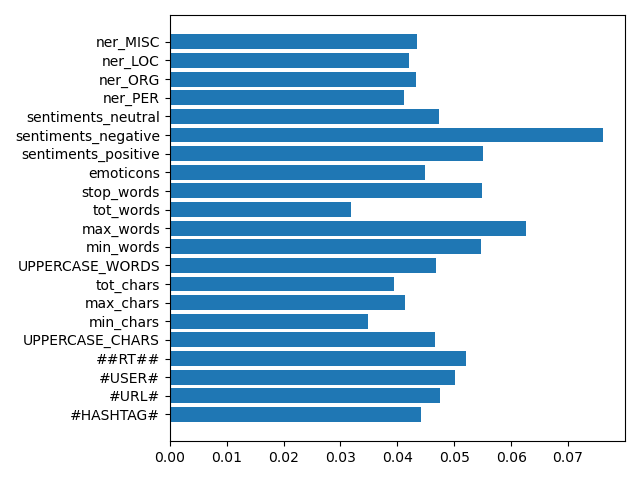
\includegraphics[width=0.75\textwidth]{assets/img/xgb_imp.png}
         \caption{\ac{XGB}}
         \label{fig:results:feat-imp::xgb}
         \vspace{0.6cm}
     \end{subfigure}
     \hfill
     \begin{subfigure}[b]{0.48\textwidth}
         \centering
         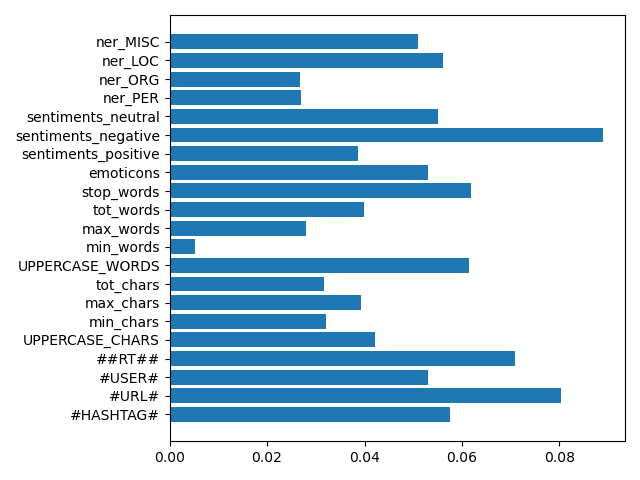
\includegraphics[width=\textwidth]{assets/img/rf_imp.png}
         \caption{\ac{RF}}
         \label{fig:results:feat-imp::rf}
     \end{subfigure}
     \hfill
     \begin{subfigure}[b]{0.48\textwidth}
         \centering
         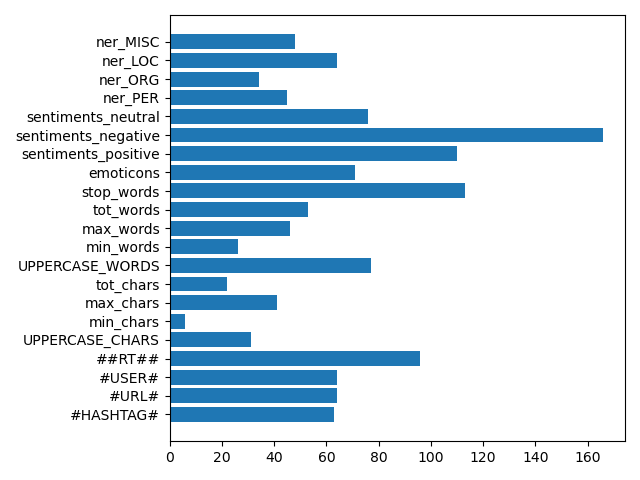
\includegraphics[width=\textwidth]{assets/img/lgb_imp.png}
         \caption{\ac{LGBM}}
         \label{fig:results:feat-imp::lgbm}
     \end{subfigure}
        \caption[Feature importance from trained \texorpdfstring{XGB}{XGB}, \texorpdfstring{RF}{RF} and \texorpdfstring{LGBM}{LGBM} models in Section \ref{sec:models:feat-based}]{Feature importance from trained \ac{XGB}, \ac{RF} and \ac{LGBM} models in Section \ref{sec:models:feat-based}}
        \label{fig:results:feat-imp}
\end{figure}
% https://tex.stackexchange.com/questions/551637/using-acronyms-in-toc

\newpage

\subsection{Word-embedding based representation}
\label{sec:results:word-emb}

% Please add the following required packages to your document preamble:
% \usepackage{multirow}
% \usepackage[table,xcdraw]{xcolor}
% If you use beamer only pass "xcolor=table" option, i.e. \documentclass[xcolor=table]{beamer}
\begin{table}[htbp]
\centering
\begin{tabular}{llrrrr}
\hline
\multicolumn{1}{l}{\textbf{Embedding}} &  & \multicolumn{1}{l}{} & \multicolumn{1}{l}{} & \multicolumn{1}{l}{} & \multicolumn{1}{l}{} \\
\multicolumn{1}{l}{\textbf{dimension}} & \multirow{-2}{*}{\textbf{Pooling}} & \multicolumn{1}{l}{\multirow{-2}{*}{\textbf{Accuracy}}} & \multicolumn{1}{l}{\multirow{-2}{*}{\textbf{Precision}}} & \multicolumn{1}{l}{\multirow{-2}{*}{\textbf{Recall}}} & \multicolumn{1}{l}{\multirow{-2}{*}{\textbf{F1-score}}} \\ \hline
 & Mean & 0.5200 & 0.5161 & 0.6400 & 0.5714 \\
 & Max. & 0.5200 & 0.5179 & 0.5800 & 0.5472 \\
 & Min. & 0.5500 & 0.5455 & 0.6000 & 0.5714 \\
\multirow{-4}{*}{25} & Abs. Max. & 0.5500 & 0.5556 & 0.5000 & 0.5263 \\ \hline
 & Mean & 0.4900 & 0.4923 & 0.6400 & 0.5565 \\
 & Max. & 0.4500 & 0.4444 & 0.4000 & 0.4211 \\
 & Min. & 0.5000 & 0.5000 & 0.5200 & 0.5098 \\
\multirow{-4}{*}{200} & Abs. Max. & 0.5100 & 0.5091 & 0.5600 & 0.5333 \\ \hline
\end{tabular}
\caption{Performance of models trained with Word-embedding based representation (Section \ref{sec:models:word-emb-based})}
\label{tab:results:performance-word-emb-based}
\end{table}


From Table \ref{tab:results:performance-word-emb-based}, we can observe that the models' performances are worse than the previous two setups. The fact that the training set is small (only 200 examples in training set) could be one of the reasons for not being able to train robust deep learning models from scratch.



\chapter{CONCLUSION AND FUTURE WORKS}
\label{chap:future-works}
We focused on identifying those user accounts on Twitter that are keen to spread Hate Speech in this work.
We described the dataset used and performed an exploratory data analysis in Chapter \ref{chap:dataset}. We also extracted several features, such as user and stylistic features, sentiments, emoticons, stopwords and named-entity mentions, and their several statistical properties. We used them for constructing baselines in the later sections.  

In Chapter \ref{chap:models}, we built some baselines and proposed a novel model. The baselines included: (i) using the term frequencies (like \ac{TF-IDF} Vectorization) to obtain user representation from the tweet texts; (ii) using the handcrafted features to construct the user representation; (iii) using the \ac{GloVe} word embeddings to represent tweets and an \ac{LSTM} for classification; and (iv) using a two-stage system to flag the user as Hate Speech Spreader if the number of hate containing tweets is beyond a certain threshold.
Our proposed model leveraged the pre-trained word embeddings for encoding the words and incorporated the sentiment scores as weights to mark the importance of the words. It computed a weighted sum to get the tweet representation and aggregated these to obtain the user representation, which was finally fed to an ML classifier like \ac{LR}, \ac{SVM}, \ac{RF}, \ac{XGB}, \ac{LGBM} or \ac{NN}. Finally, we constructed a max-voting classifier (ensemble) using the different models.

We discussed the performance of different models in Chapter \ref{chap:results}. The best accuracy we obtained with the baseline models was 69\%. We also observed that the ``negative sentiment'' score had the highest feature importance in baselines developed using the handcrafted features (Section \ref{sec:results:feat-extr}), which further motivated us to work towards our proposed model. Our model achieved an accuracy of 76\% on the test set, which was 1\% more than the best performance obtained in the competition. The ensemble model consisting of \ac{TF-IDF}+\ac{LR}, \ac{RoBERTa} and \ac{LR} classifier with 25d \ac{GloVe} word embeddings from Sections \ref{sec:models:tf-idf}, \ref{sec:models:count-hate} and \ref{sec:models:our-model} achieved an accuracy of 77\%, a further 1\% increase. Finally, we performed an error analysis where we discussed some limitations of our model.

In the future, we plan to conduct a deeper analysis of the results and investigate these models in more detail. We would also like to address some of the limitations discussed in Section \ref{sec:results:err-ana}.


% Clearly, the fine-tuned  model and the  have the best performance in Section \ref{sec:results:count-hate} and Section \ref{sec:results:our-model}, respectively. However, since both \ac{TF-IDF}+\ac{LR} and \ac{TF-IDF}+\ac{SVM} have the same test accuracy in Section , 


% While it is intuitive that tweets indicating hate tend to carry a high negative sentiment score, our experiments also show that the negative sentiment score is the most important feature among all other features considered. Our model achieves an accuracy of 76\% on the test set and outperforms the best model in the competition. We further improve the accuracy by creating an ensemble of models. In future, we plan to investigate these models in more detail.

% , developed several baselines in Chapter \ref{chap:models} and discussed their results in Chapter \ref{chap:results}. We obtained the best accuracy of 69\% on the test set, which is six points lower than the best performing model on English tweets. However, these models did not make use of any external knowledge. The pre-processing pipeline was also kept simple and had minimal steps (for instance, we did not use any internet slang dictionary, emotional quotient features, spelling correction, etc.).

% We also observed in Section \ref{sec:results:feat-extr} that the ``negative sentiment'' feature has the highest importance among the different features. We also linked it to the characteristic of the Hate Speech itself, i.e., since it implies abuse or harm, it must have a high negative sentiment score. We plan to exploit this observation in our future works.

% As the next step, we plan to assign weights to words that appear in the tweets based on the sentiment score after removing stop words and take a weighted average of the word embeddings\eat{, in contrast to the simple average in our baselines,} to get the user-level representation for classification.

% feature selection in feature-based baseline
% word embeddings
% using sentiment

% - hate degree, frequency, ...

% - HatEval2019 and Zerak datasets
%     - baselines
%     - ensemble
%     - sota models (also low)
%     - feature importance

% - thresholding





% \begin{itemize}

% \item For special figure captions the \texttt{ccaption} package may be
%   useful.  This is specially useful if one has a figure that spans
%   more than two pages and you need to use the same figure number.

% \item The notation page can be entered manually or automatically
%   generated using the \texttt{nomencl} package.

% \end{itemize}


%%%%%%%%%%%%%%%%%%%%%%%%%%%%%%%%%%%%%%%%%%%%%%%%%%%%%%%%%%%%
% Appendices.

\appendix

% \chapter{VALUES CORRESPONDING TO DIFFERENT EXTRACTED FEATURES FOR EACH USER}
% \label{chap:per-user-stats}
% \sdcomment{TODO: not sure how to fit 21 columns in one page...}


% Please add the following required packages to your document preamble:
% \usepackage{lscape}
% \usepackage{longtable}
% Note: It may be necessary to compile the document several times to get a multi-page table to line up properly
\small{
\begin{landscape}
\begin{longtable}[c]{lrrrrrrrrrrrrrrrrrrrrr}
\hline
\textbf{label} & \textbf{hash} & \textbf{urls} & \textbf{users} & \textbf{rt} & \textbf{UP\_} & \textbf{min\_} & \textbf{max\_} & \textbf{tot\_} & \textbf{UP\_} & \textbf{min\_} & \textbf{max\_} & \textbf{tot\_} & \textbf{stop\_} & \textbf{emoticons} & \textbf{senti\_} & \textbf{senti\_} & \textbf{senti\_} & \textbf{ner\_} & \textbf{ner\_} & \textbf{ner\_} & \textbf{ner\_} \\
& \textbf{tags} &  &  &  & \textbf{chars} & \textbf{chars} & \textbf{chars} & \textbf{chars} & \textbf{words} & \textbf{words} & \textbf{words} & \textbf{words} & \textbf{words} &  & \textbf{+ve} & \textbf{-ve} & \textbf{0} & \textbf{PER} & \textbf{ORG} & \textbf{LOC} & \textbf{MISC} \\

\hline
\endhead
%
0 & 10 & 92 & 22 & 195 & 1245 & 11 & 122 & 14535 & 891 & 3 & 24 & 2553 & 959 & 15 & 46 & 42 & 112 & 99 & 50 & 36 & 95 \\
0 & 14 & 121 & 140 & 34 & 1798 & 9 & 121 & 10369 & 650 & 4 & 25 & 2137 & 814 & 321 & 40 & 27 & 133 & 55 & 33 & 19 & 103 \\
0 & 19 & 99 & 253 & 73 & 457 & 13 & 140 & 12253 & 356 & 4 & 26 & 2576 & 1137 & 22 & 71 & 31 & 98 & 38 & 13 & 24 & 29 \\
0 & 35 & 63 & 168 & 103 & 863 & 10 & 127 & 13290 & 557 & 3 & 24 & 2576 & 1055 & 53 & 60 & 57 & 83 & 76 & 51 & 38 & 66 \\
0 & 0 & 22 & 213 & 3 & 496 & 13 & 139 & 14768 & 395 & 4 & 32 & 3177 & 1520 & 11 & 82 & 50 & 68 & 53 & 28 & 36 & 42 \\
0 & 33 & 113 & 114 & 23 & 689 & 4 & 117 & 8594 & 315 & 2 & 26 & 1968 & 721 & 152 & 73 & 17 & 110 & 61 & 12 & 18 & 79 \\
0 & 76 & 110 & 84 & 136 & 999 & 7 & 134 & 11820 & 624 & 3 & 27 & 2432 & 976 & 53 & 79 & 20 & 101 & 40 & 24 & 29 & 78 \\
0 & 39 & 118 & 36 & 151 & 645 & 4 & 117 & 7685 & 340 & 2 & 27 & 1683 & 619 & 123 & 43 & 25 & 132 & 61 & 15 & 15 & 68 \\
0 & 0 & 7 & 3 & 45 & 525 & 9 & 128 & 9892 & 218 & 3 & 28 & 2121 & 1145 & 85 & 65 & 49 & 86 & 29 & 7 & 8 & 44 \\
0 & 0 & 196 & 0 & 1 & 6 & 28 & 79 & 12431 & 3 & 6 & 15 & 2271 & 725 & 1 & 1 & 1 & 198 & 0 & 0 & 0 & 0 \\
0 & 9 & 25 & 12 & 41 & 468 & 6 & 134 & 10890 & 235 & 3 & 28 & 2361 & 1103 & 149 & 44 & 41 & 115 & 28 & 16 & 6 & 45 \\
0 & 1 & 35 & 18 & 123 & 143 & 11 & 135 & 9441 & 79 & 3 & 30 & 2049 & 1034 & 218 & 72 & 44 & 84 & 25 & 12 & 7 & 31 \\
0 & 0 & 11 & 13 & 11 & 391 & 9 & 128 & 11262 & 175 & 3 & 29 & 2349 & 1067 & 186 & 65 & 50 & 85 & 28 & 5 & 9 & 48 \\
0 & 0 & 205 & 57 & 1 & 1235 & 18 & 116 & 13766 & 844 & 5 & 22 & 2476 & 651 & 0 & 35 & 35 & 130 & 49 & 104 & 111 & 137 \\
0 & 30 & 12 & 110 & 38 & 361 & 11 & 135 & 8843 & 264 & 3 & 25 & 1907 & 803 & 248 & 65 & 36 & 99 & 33 & 5 & 11 & 51 \\
0 & 0 & 57 & 11 & 85 & 437 & 12 & 125 & 13765 & 219 & 3 & 28 & 2767 & 1475 & 110 & 108 & 40 & 52 & 27 & 17 & 47 & 36 \\
0 & 2 & 19 & 3 & 184 & 845 & 10 & 122 & 11733 & 338 & 3 & 24 & 2379 & 1160 & 164 & 66 & 44 & 90 & 38 & 14 & 11 & 80 \\
0 & 1 & 19 & 27 & 29 & 360 & 5 & 123 & 8498 & 219 & 1 & 22 & 1801 & 913 & 48 & 78 & 35 & 87 & 29 & 8 & 17 & 33 \\
0 & 13 & 38 & 110 & 32 & 370 & 10 & 140 & 11473 & 295 & 3 & 27 & 2383 & 1106 & 71 & 71 & 44 & 85 & 42 & 10 & 21 & 43 \\
0 & 0 & 43 & 11 & 85 & 475 & 14 & 132 & 10412 & 242 & 3 & 31 & 2139 & 1045 & 119 & 66 & 39 & 95 & 33 & 6 & 11 & 48 \\
0 & 1 & 47 & 11 & 114 & 310 & 4 & 111 & 10705 & 189 & 2 & 25 & 2245 & 1159 & 93 & 74 & 46 & 80 & 33 & 12 & 15 & 49 \\
0 & 5 & 37 & 37 & 31 & 354 & 9 & 116 & 7693 & 249 & 3 & 22 & 1642 & 692 & 70 & 51 & 35 & 114 & 52 & 7 & 6 & 36 \\
0 & 12 & 21 & 203 & 28 & 507 & 11 & 128 & 10901 & 353 & 3 & 27 & 2271 & 1135 & 4 & 102 & 28 & 70 & 36 & 10 & 17 & 34 \\
0 & 28 & 94 & 60 & 87 & 651 & 11 & 140 & 9644 & 358 & 3 & 30 & 2152 & 967 & 243 & 64 & 32 & 104 & 50 & 14 & 5 & 70 \\
0 & 0 & 50 & 31 & 47 & 317 & 8 & 140 & 10055 & 174 & 3 & 29 & 2208 & 1014 & 374 & 52 & 52 & 96 & 32 & 12 & 10 & 39 \\
0 & 1 & 60 & 99 & 6 & 371 & 9 & 138 & 10254 & 211 & 3 & 29 & 2272 & 970 & 176 & 61 & 60 & 79 & 45 & 7 & 6 & 35 \\
0 & 0 & 93 & 3 & 179 & 793 & 12 & 136 & 10073 & 289 & 4 & 25 & 2148 & 1066 & 141 & 50 & 43 & 107 & 33 & 19 & 9 & 69 \\
0 & 5 & 67 & 155 & 16 & 503 & 9 & 137 & 9693 & 213 & 4 & 27 & 2089 & 946 & 23 & 78 & 31 & 91 & 29 & 17 & 12 & 57 \\
0 & 9 & 5 & 1 & 174 & 483 & 9 & 120 & 11839 & 196 & 3 & 28 & 2471 & 1329 & 96 & 77 & 61 & 62 & 21 & 13 & 5 & 36 \\
0 & 4 & 153 & 18 & 25 & 132 & 11 & 99 & 9893 & 91 & 3 & 22 & 1949 & 729 & 77 & 25 & 27 & 148 & 13 & 2 & 3 & 12 \\
0 & 2 & 55 & 67 & 65 & 492 & 9 & 143 & 8864 & 270 & 3 & 28 & 1998 & 791 & 227 & 75 & 30 & 95 & 31 & 8 & 4 & 65 \\
0 & 0 & 11 & 343 & 4 & 356 & 9 & 121 & 10765 & 280 & 4 & 23 & 2168 & 917 & 0 & 57 & 32 & 111 & 33 & 12 & 17 & 37 \\
0 & 8 & 102 & 8 & 86 & 554 & 7 & 132 & 9910 & 284 & 3 & 29 & 2120 & 972 & 129 & 51 & 55 & 94 & 43 & 21 & 14 & 57 \\
0 & 58 & 4 & 232 & 1 & 254 & 10 & 134 & 12269 & 227 & 4 & 28 & 2820 & 1340 & 25 & 67 & 61 & 72 & 23 & 25 & 14 & 33 \\
0 & 2 & 51 & 45 & 71 & 567 & 11 & 132 & 10852 & 302 & 3 & 28 & 2311 & 1103 & 170 & 58 & 42 & 100 & 46 & 15 & 8 & 58 \\
0 & 0 & 34 & 66 & 42 & 549 & 12 & 140 & 11970 & 356 & 4 & 29 & 2387 & 1173 & 48 & 71 & 38 & 91 & 45 & 24 & 17 & 50 \\
0 & 20 & 60 & 149 & 77 & 490 & 10 & 139 & 10895 & 247 & 3 & 26 & 2368 & 1096 & 261 & 72 & 43 & 85 & 49 & 10 & 9 & 68 \\
0 & 16 & 66 & 69 & 68 & 580 & 11 & 120 & 9331 & 314 & 3 & 25 & 1916 & 864 & 120 & 65 & 49 & 86 & 39 & 13 & 20 & 42 \\
0 & 10 & 29 & 70 & 23 & 409 & 5 & 121 & 8085 & 209 & 3 & 26 & 1824 & 772 & 143 & 60 & 37 & 103 & 31 & 10 & 14 & 46 \\
0 & 11 & 44 & 92 & 141 & 1906 & 10 & 127 & 12028 & 721 & 3 & 27 & 2575 & 949 & 413 & 95 & 30 & 75 & 32 & 51 & 16 & 110 \\
0 & 13 & 30 & 66 & 44 & 294 & 7 & 93 & 7835 & 173 & 3 & 24 & 1761 & 764 & 95 & 51 & 39 & 110 & 45 & 9 & 7 & 42 \\
0 & 7 & 80 & 37 & 120 & 550 & 13 & 124 & 10025 & 313 & 3 & 25 & 2164 & 1009 & 135 & 76 & 29 & 95 & 59 & 21 & 12 & 59 \\
0 & 8 & 160 & 17 & 188 & 726 & 8 & 121 & 9117 & 348 & 3 & 23 & 1990 & 833 & 244 & 61 & 38 & 101 & 49 & 24 & 14 & 50 \\
0 & 2 & 85 & 9 & 174 & 693 & 8 & 125 & 10800 & 317 & 3 & 27 & 2250 & 1045 & 166 & 54 & 52 & 94 & 40 & 18 & 8 & 56 \\
0 & 6 & 70 & 14 & 86 & 753 & 12 & 136 & 10403 & 346 & 4 & 28 & 2092 & 955 & 168 & 74 & 36 & 90 & 43 & 17 & 13 & 61 \\
0 & 2 & 92 & 12 & 161 & 479 & 12 & 122 & 10091 & 221 & 3 & 24 & 2086 & 949 & 119 & 54 & 48 & 98 & 37 & 19 & 12 & 47 \\
0 & 533 & 194 & 0 & 0 & 682 & 17 & 112 & 10233 & 540 & 3 & 22 & 2524 & 795 & 0 & 65 & 19 & 116 & 101 & 31 & 25 & 69 \\
0 & 2 & 11 & 177 & 0 & 505 & 7 & 140 & 9142 & 311 & 4 & 28 & 1998 & 967 & 94 & 68 & 30 & 102 & 36 & 9 & 7 & 46 \\
0 & 4 & 87 & 7 & 195 & 714 & 11 & 119 & 10105 & 381 & 3 & 25 & 2077 & 1006 & 136 & 72 & 25 & 103 & 41 & 19 & 9 & 85 \\
0 & 1 & 67 & 69 & 43 & 497 & 10 & 139 & 12217 & 229 & 3 & 28 & 2537 & 1265 & 45 & 62 & 51 & 87 & 38 & 22 & 11 & 48 \\
0 & 0 & 8 & 267 & 0 & 1268 & 18 & 141 & 16917 & 746 & 4 & 26 & 3102 & 1169 & 9 & 70 & 56 & 74 & 75 & 43 & 52 & 102 \\
0 & 2 & 83 & 24 & 158 & 620 & 10 & 133 & 11929 & 320 & 3 & 29 & 2427 & 1207 & 225 & 52 & 50 & 98 & 31 & 8 & 15 & 77 \\
0 & 4 & 56 & 48 & 140 & 539 & 11 & 124 & 10779 & 310 & 3 & 27 & 2177 & 1036 & 65 & 81 & 32 & 87 & 36 & 20 & 13 & 42 \\
0 & 8 & 53 & 167 & 81 & 468 & 10 & 118 & 10505 & 277 & 3 & 23 & 2251 & 980 & 17 & 65 & 46 & 89 & 52 & 7 & 26 & 57 \\
0 & 11 & 61 & 104 & 34 & 571 & 10 & 136 & 11066 & 193 & 3 & 27 & 2266 & 973 & 22 & 71 & 39 & 90 & 31 & 28 & 9 & 47 \\
0 & 57 & 60 & 227 & 4 & 589 & 8 & 123 & 10673 & 410 & 4 & 23 & 2208 & 985 & 1 & 77 & 34 & 89 & 24 & 29 & 36 & 57 \\
0 & 285 & 185 & 21 & 16 & 392 & 9 & 112 & 9488 & 343 & 4 & 22 & 2135 & 785 & 6 & 61 & 40 & 99 & 37 & 24 & 17 & 42 \\
0 & 20 & 206 & 92 & 0 & 2248 & 24 & 113 & 14373 & 1874 & 5 & 21 & 2639 & 702 & 0 & 58 & 24 & 118 & 69 & 71 & 30 & 194 \\
0 & 1 & 129 & 0 & 0 & 862 & 12 & 141 & 11109 & 702 & 3 & 25 & 2115 & 664 & 27 & 129 & 8 & 63 & 66 & 53 & 50 & 124 \\
0 & 11 & 122 & 122 & 22 & 582 & 8 & 126 & 11400 & 427 & 4 & 25 & 2389 & 1000 & 14 & 65 & 46 & 89 & 46 & 26 & 31 & 50 \\
0 & 0 & 176 & 291 & 31 & 2525 & 14 & 124 & 12743 & 1319 & 4 & 25 & 2598 & 808 & 164 & 34 & 32 & 134 & 60 & 66 & 26 & 123 \\
0 & 5 & 81 & 293 & 14 & 667 & 13 & 123 & 12226 & 546 & 4 & 23 & 2440 & 934 & 44 & 69 & 29 & 102 & 55 & 26 & 44 & 77 \\
0 & 18 & 127 & 109 & 127 & 788 & 10 & 115 & 9529 & 377 & 4 & 24 & 2053 & 850 & 20 & 75 & 36 & 89 & 45 & 15 & 2 & 62 \\
0 & 7 & 154 & 36 & 51 & 1053 & 7 & 140 & 10980 & 488 & 3 & 25 & 2111 & 897 & 38 & 82 & 23 & 95 & 27 & 56 & 16 & 96 \\
0 & 312 & 85 & 105 & 73 & 1044 & 12 & 124 & 10697 & 599 & 4 & 22 & 2342 & 670 & 59 & 54 & 38 & 108 & 69 & 118 & 23 & 65 \\
0 & 213 & 154 & 32 & 61 & 790 & 10 & 114 & 12233 & 647 & 3 & 24 & 2478 & 823 & 8 & 60 & 26 & 114 & 83 & 43 & 49 & 73 \\
0 & 101 & 193 & 152 & 6 & 664 & 12 & 121 & 10705 & 526 & 4 & 23 & 2305 & 862 & 41 & 61 & 40 & 99 & 31 & 30 & 31 & 69 \\
0 & 13 & 37 & 224 & 44 & 428 & 9 & 125 & 8730 & 324 & 1 & 25 & 2009 & 752 & 235 & 56 & 35 & 109 & 48 & 14 & 28 & 63 \\
0 & 5 & 67 & 50 & 169 & 1024 & 11 & 121 & 13144 & 749 & 3 & 25 & 2514 & 1130 & 30 & 60 & 40 & 100 & 80 & 39 & 41 & 73 \\
0 & 40 & 93 & 245 & 94 & 648 & 12 & 121 & 12610 & 463 & 4 & 25 & 2689 & 1090 & 26 & 68 & 45 & 87 & 42 & 14 & 28 & 74 \\
0 & 54 & 96 & 31 & 137 & 1030 & 11 & 118 & 11277 & 699 & 3 & 23 & 2194 & 805 & 88 & 58 & 19 & 123 & 83 & 48 & 41 & 90 \\
0 & 50 & 115 & 70 & 163 & 691 & 9 & 124 & 12602 & 447 & 3 & 27 & 2503 & 969 & 132 & 54 & 47 & 99 & 55 & 26 & 56 & 71 \\
0 & 16 & 41 & 170 & 98 & 1059 & 9 & 126 & 11741 & 542 & 2 & 25 & 2393 & 1034 & 236 & 73 & 37 & 90 & 58 & 37 & 31 & 84 \\
0 & 14 & 102 & 106 & 48 & 654 & 12 & 134 & 12087 & 508 & 3 & 24 & 2302 & 1019 & 10 & 64 & 34 & 102 & 64 & 13 & 22 & 80 \\
0 & 58 & 124 & 135 & 75 & 709 & 10 & 115 & 9771 & 501 & 3 & 26 & 2170 & 778 & 95 & 79 & 22 & 99 & 58 & 22 & 34 & 101 \\
0 & 22 & 110 & 238 & 22 & 437 & 8 & 124 & 10690 & 376 & 3 & 26 & 2278 & 861 & 12 & 46 & 25 & 129 & 32 & 22 & 38 & 50 \\
0 & 24 & 96 & 107 & 139 & 717 & 11 & 138 & 12229 & 503 & 3 & 25 & 2381 & 1042 & 41 & 77 & 30 & 93 & 58 & 51 & 36 & 62 \\
0 & 36 & 99 & 152 & 121 & 700 & 7 & 120 & 11093 & 563 & 3 & 24 & 2212 & 825 & 18 & 62 & 37 & 101 & 67 & 44 & 21 & 73 \\
0 & 2 & 28 & 20 & 67 & 496 & 10 & 119 & 7689 & 167 & 3 & 24 & 1575 & 755 & 47 & 65 & 41 & 94 & 18 & 11 & 16 & 53 \\
0 & 6 & 26 & 251 & 195 & 716 & 7 & 117 & 9835 & 491 & 4 & 23 & 2124 & 981 & 36 & 62 & 26 & 112 & 43 & 18 & 13 & 59 \\
0 & 34 & 135 & 61 & 169 & 815 & 11 & 125 & 13489 & 593 & 4 & 25 & 2541 & 1037 & 16 & 74 & 35 & 91 & 50 & 24 & 43 & 72 \\
0 & 20 & 94 & 70 & 193 & 958 & 13 & 118 & 12085 & 565 & 3 & 24 & 2333 & 1000 & 64 & 57 & 20 & 123 & 81 & 50 & 27 & 64 \\
0 & 159 & 136 & 69 & 97 & 702 & 4 & 120 & 12735 & 587 & 3 & 22 & 2538 & 944 & 10 & 52 & 43 & 105 & 49 & 34 & 91 & 83 \\
0 & 1 & 64 & 97 & 19 & 1296 & 9 & 108 & 8359 & 379 & 3 & 22 & 1858 & 790 & 72 & 41 & 51 & 108 & 22 & 26 & 6 & 65 \\
0 & 63 & 86 & 105 & 144 & 945 & 12 & 128 & 14126 & 613 & 4 & 26 & 2675 & 1061 & 47 & 80 & 33 & 87 & 54 & 42 & 50 & 79 \\
0 & 58 & 103 & 69 & 160 & 1049 & 8 & 133 & 11505 & 599 & 3 & 21 & 2210 & 909 & 120 & 59 & 30 & 111 & 49 & 36 & 22 & 72 \\
0 & 12 & 24 & 245 & 10 & 411 & 9 & 133 & 9392 & 321 & 4 & 30 & 2089 & 862 & 158 & 42 & 55 & 103 & 24 & 29 & 14 & 65 \\
0 & 30 & 87 & 197 & 101 & 730 & 7 & 127 & 12175 & 544 & 3 & 26 & 2463 & 1003 & 8 & 66 & 42 & 92 & 74 & 33 & 24 & 53 \\
0 & 28 & 118 & 101 & 173 & 762 & 11 & 121 & 12938 & 616 & 3 & 24 & 2455 & 920 & 32 & 66 & 35 & 99 & 89 & 31 & 44 & 66 \\
0 & 163 & 213 & 101 & 2 & 752 & 9 & 106 & 12371 & 580 & 3 & 24 & 2560 & 823 & 21 & 79 & 28 & 93 & 38 & 35 & 48 & 81 \\
0 & 0 & 192 & 13 & 0 & 1057 & 14 & 126 & 12819 & 893 & 4 & 23 & 2374 & 763 & 4 & 54 & 32 & 114 & 49 & 37 & 129 & 113 \\
0 & 60 & 121 & 287 & 35 & 886 & 10 & 119 & 10121 & 599 & 3 & 22 & 2272 & 834 & 3 & 49 & 37 & 114 & 31 & 29 & 19 & 55 \\
0 & 2 & 89 & 92 & 127 & 1182 & 12 & 134 & 13481 & 644 & 3 & 26 & 2506 & 1046 & 22 & 73 & 33 & 94 & 91 & 51 & 28 & 84 \\
0 & 25 & 138 & 123 & 134 & 1167 & 11 & 122 & 11133 & 673 & 3 & 24 & 2223 & 808 & 48 & 55 & 30 & 115 & 65 & 36 & 26 & 79 \\
0 & 49 & 99 & 148 & 2 & 476 & 11 & 129 & 12857 & 398 & 4 & 26 & 2536 & 1168 & 48 & 78 & 42 & 80 & 44 & 12 & 30 & 58 \\
0 & 24 & 86 & 98 & 99 & 848 & 12 & 117 & 14638 & 619 & 4 & 26 & 2839 & 1349 & 20 & 63 & 46 & 91 & 74 & 38 & 31 & 89 \\
0 & 172 & 139 & 60 & 94 & 984 & 7 & 117 & 11686 & 763 & 4 & 22 & 2393 & 839 & 12 & 43 & 38 & 119 & 64 & 47 & 22 & 92 \\
0 & 31 & 154 & 45 & 162 & 707 & 9 & 123 & 12806 & 498 & 3 & 23 & 2432 & 987 & 8 & 60 & 39 & 101 & 55 & 36 & 55 & 57 \\
0 & 0 & 2 & 212 & 0 & 261 & 10 & 121 & 9145 & 140 & 4 & 26 & 2095 & 1103 & 36 & 60 & 27 & 113 & 5 & 4 & 0 & 40 \\
0 & 379 & 160 & 69 & 33 & 779 & 9 & 132 & 9661 & 552 & 4 & 32 & 2354 & 766 & 93 & 74 & 20 & 106 & 72 & 38 & 40 & 79 \\
1 & 88 & 163 & 155 & 37 & 1406 & 8 & 127 & 11304 & 682 & 4 & 25 & 2390 & 956 & 1 & 45 & 61 & 94 & 38 & 32 & 16 & 113 \\
1 & 12 & 13 & 143 & 0 & 505 & 17 & 140 & 16135 & 399 & 5 & 30 & 3319 & 1485 & 28 & 75 & 44 & 81 & 95 & 30 & 53 & 73 \\
1 & 16 & 131 & 138 & 59 & 578 & 10 & 116 & 9823 & 358 & 4 & 25 & 2159 & 840 & 34 & 63 & 54 & 83 & 60 & 27 & 14 & 46 \\
1 & 6 & 2 & 177 & 1 & 380 & 10 & 135 & 8159 & 112 & 3 & 27 & 1854 & 705 & 57 & 49 & 54 & 97 & 11 & 10 & 6 & 40 \\
1 & 29 & 91 & 52 & 6 & 909 & 10 & 140 & 11444 & 666 & 3 & 27 & 2221 & 926 & 69 & 66 & 36 & 98 & 85 & 15 & 15 & 84 \\
1 & 103 & 0 & 0 & 0 & 2881 & 56 & 140 & 19802 & 890 & 9 & 32 & 3910 & 2061 & 0 & 76 & 54 & 70 & 27 & 56 & 15 & 179 \\
1 & 2 & 26 & 1 & 55 & 376 & 13 & 134 & 12031 & 201 & 4 & 27 & 2477 & 1225 & 94 & 62 & 61 & 77 & 28 & 15 & 7 & 26 \\
1 & 9 & 23 & 28 & 32 & 398 & 8 & 140 & 10781 & 211 & 3 & 30 & 2393 & 1015 & 243 & 69 & 42 & 89 & 35 & 12 & 4 & 64 \\
1 & 1 & 24 & 13 & 36 & 398 & 10 & 131 & 10439 & 195 & 3 & 25 & 2204 & 1135 & 117 & 46 & 59 & 95 & 39 & 13 & 5 & 41 \\
1 & 102 & 22 & 177 & 9 & 176 & 14 & 128 & 10723 & 134 & 4 & 25 & 2452 & 940 & 320 & 77 & 61 & 62 & 43 & 11 & 16 & 26 \\
1 & 0 & 53 & 19 & 69 & 245 & 8 & 119 & 8586 & 140 & 3 & 25 & 1861 & 833 & 215 & 69 & 45 & 86 & 39 & 7 & 16 & 30 \\
1 & 0 & 14 & 13 & 155 & 279 & 11 & 127 & 9067 & 103 & 3 & 26 & 1927 & 951 & 221 & 62 & 56 & 82 & 29 & 12 & 4 & 31 \\
1 & 168 & 4 & 120 & 0 & 967 & 9 & 135 & 12340 & 469 & 3 & 28 & 2678 & 1240 & 3 & 46 & 105 & 49 & 37 & 40 & 9 & 74 \\
1 & 16 & 17 & 305 & 21 & 674 & 11 & 132 & 10346 & 469 & 4 & 26 & 2375 & 1062 & 3 & 56 & 67 & 77 & 74 & 13 & 12 & 72 \\
1 & 8 & 14 & 47 & 14 & 366 & 10 & 125 & 8621 & 283 & 3 & 29 & 1820 & 795 & 54 & 53 & 46 & 101 & 67 & 25 & 12 & 36 \\
1 & 0 & 66 & 18 & 101 & 509 & 9 & 124 & 9920 & 234 & 3 & 25 & 2125 & 1061 & 100 & 67 & 46 & 87 & 38 & 7 & 12 & 40 \\
1 & 0 & 0 & 0 & 0 & 543 & 19 & 140 & 14157 & 504 & 4 & 30 & 2742 & 1126 & 31 & 82 & 63 & 55 & 73 & 18 & 7 & 111 \\
1 & 1 & 10 & 30 & 125 & 267 & 10 & 125 & 9789 & 98 & 4 & 26 & 2082 & 1045 & 129 & 62 & 52 & 86 & 17 & 14 & 5 & 43 \\
1 & 2 & 11 & 17 & 96 & 395 & 10 & 130 & 9871 & 158 & 3 & 26 & 2090 & 1029 & 180 & 62 & 51 & 87 & 24 & 13 & 10 & 39 \\
1 & 44 & 13 & 84 & 20 & 1238 & 11 & 140 & 11922 & 427 & 3 & 28 & 2426 & 1105 & 0 & 77 & 57 & 66 & 29 & 21 & 12 & 51 \\
1 & 10 & 46 & 66 & 42 & 384 & 9 & 106 & 7936 & 224 & 3 & 17 & 1818 & 840 & 149 & 51 & 40 & 109 & 37 & 25 & 11 & 40 \\
1 & 1 & 31 & 47 & 98 & 422 & 10 & 139 & 10019 & 201 & 4 & 31 & 2167 & 1104 & 206 & 61 & 53 & 86 & 33 & 4 & 11 & 48 \\
1 & 2 & 20 & 31 & 28 & 461 & 11 & 136 & 11573 & 280 & 3 & 29 & 2492 & 1220 & 117 & 55 & 46 & 99 & 44 & 24 & 13 & 44 \\
1 & 7 & 48 & 23 & 53 & 460 & 5 & 126 & 9173 & 223 & 2 & 25 & 1901 & 873 & 289 & 47 & 33 & 120 & 33 & 8 & 9 & 56 \\
1 & 0 & 23 & 13 & 161 & 239 & 11 & 120 & 9648 & 104 & 3 & 25 & 2017 & 1016 & 60 & 66 & 43 & 91 & 18 & 9 & 13 & 32 \\
1 & 5 & 87 & 16 & 52 & 441 & 7 & 115 & 8806 & 201 & 3 & 20 & 1804 & 696 & 83 & 30 & 30 & 140 & 22 & 9 & 8 & 33 \\
1 & 3 & 71 & 39 & 72 & 472 & 9 & 120 & 8915 & 277 & 4 & 26 & 1915 & 834 & 316 & 53 & 46 & 101 & 44 & 14 & 17 & 58 \\
1 & 1 & 62 & 62 & 15 & 507 & 10 & 144 & 10883 & 252 & 3 & 31 & 2370 & 1092 & 118 & 105 & 40 & 55 & 58 & 14 & 15 & 49 \\
1 & 1 & 69 & 13 & 64 & 262 & 11 & 125 & 10046 & 107 & 3 & 27 & 2158 & 995 & 164 & 58 & 55 & 87 & 28 & 14 & 9 & 47 \\
1 & 16 & 11 & 298 & 4 & 350 & 11 & 125 & 9850 & 252 & 3 & 26 & 2209 & 1008 & 38 & 61 & 38 & 101 & 29 & 10 & 12 & 40 \\
1 & 1 & 63 & 102 & 7 & 714 & 10 & 128 & 11353 & 357 & 3 & 27 & 2377 & 1145 & 101 & 67 & 55 & 78 & 38 & 10 & 11 & 61 \\
1 & 2 & 53 & 72 & 96 & 696 & 11 & 139 & 10374 & 371 & 3 & 31 & 2232 & 955 & 204 & 45 & 65 & 90 & 49 & 17 & 9 & 78 \\
1 & 3 & 69 & 22 & 57 & 361 & 9 & 128 & 9799 & 162 & 3 & 26 & 2041 & 877 & 27 & 69 & 54 & 77 & 65 & 7 & 10 & 45 \\
1 & 5 & 94 & 99 & 43 & 372 & 9 & 136 & 9215 & 261 & 3 & 28 & 2034 & 903 & 52 & 56 & 37 & 107 & 44 & 8 & 15 & 34 \\
1 & 5 & 57 & 24 & 142 & 476 & 9 & 121 & 11082 & 296 & 2 & 24 & 2253 & 1093 & 83 & 57 & 44 & 99 & 61 & 14 & 19 & 51 \\
1 & 0 & 80 & 44 & 46 & 422 & 8 & 123 & 9798 & 231 & 3 & 26 & 2116 & 998 & 23 & 72 & 58 & 70 & 33 & 9 & 7 & 32 \\
1 & 16 & 13 & 319 & 8 & 490 & 11 & 123 & 10655 & 393 & 4 & 25 & 2271 & 975 & 109 & 67 & 42 & 91 & 35 & 19 & 21 & 41 \\
1 & 0 & 46 & 25 & 101 & 627 & 8 & 117 & 7959 & 342 & 3 & 25 & 1728 & 816 & 26 & 53 & 48 & 99 & 34 & 14 & 5 & 51 \\
1 & 5 & 68 & 47 & 107 & 392 & 10 & 130 & 10345 & 239 & 3 & 29 & 2134 & 934 & 87 & 56 & 53 & 91 & 27 & 17 & 10 & 50 \\
1 & 5 & 78 & 90 & 57 & 391 & 7 & 123 & 8556 & 239 & 3 & 25 & 1853 & 851 & 104 & 55 & 37 & 108 & 45 & 13 & 16 & 41 \\
1 & 0 & 82 & 16 & 130 & 460 & 8 & 134 & 9479 & 251 & 4 & 27 & 2032 & 915 & 68 & 49 & 31 & 120 & 34 & 12 & 28 & 42 \\
1 & 5 & 99 & 36 & 143 & 864 & 11 & 122 & 9923 & 406 & 3 & 26 & 2077 & 823 & 175 & 66 & 36 & 98 & 56 & 28 & 15 & 76 \\
1 & 3 & 82 & 83 & 39 & 573 & 7 & 139 & 11988 & 435 & 4 & 27 & 2415 & 1184 & 49 & 67 & 33 & 100 & 47 & 10 & 21 & 65 \\
1 & 0 & 3 & 353 & 0 & 535 & 12 & 129 & 11854 & 462 & 4 & 29 & 2574 & 1145 & 139 & 48 & 53 & 99 & 79 & 16 & 29 & 71 \\
1 & 3 & 20 & 10 & 104 & 752 & 10 & 143 & 11637 & 268 & 3 & 30 & 2455 & 1238 & 100 & 73 & 62 & 65 & 34 & 13 & 2 & 56 \\
1 & 1 & 115 & 116 & 3 & 1128 & 10 & 120 & 15852 & 922 & 3 & 24 & 2945 & 982 & 29 & 58 & 58 & 84 & 120 & 75 & 54 & 111 \\
1 & 10 & 23 & 172 & 85 & 726 & 7 & 122 & 10728 & 432 & 3 & 24 & 2175 & 1011 & 50 & 44 & 53 & 103 & 49 & 24 & 26 & 62 \\
1 & 1 & 9 & 254 & 17 & 639 & 11 & 134 & 12533 & 503 & 4 & 25 & 2553 & 1263 & 0 & 53 & 50 & 97 & 57 & 39 & 19 & 49 \\
1 & 17 & 43 & 352 & 5 & 634 & 10 & 126 & 11169 & 303 & 4 & 22 & 2331 & 1001 & 110 & 58 & 53 & 89 & 23 & 33 & 27 & 46 \\
1 & 88 & 121 & 9 & 6 & 759 & 11 & 148 & 17723 & 592 & 4 & 29 & 3445 & 1446 & 87 & 56 & 94 & 50 & 52 & 20 & 18 & 112 \\
1 & 4 & 84 & 123 & 45 & 361 & 7 & 123 & 10884 & 305 & 3 & 27 & 2263 & 1138 & 7 & 56 & 43 & 101 & 43 & 10 & 17 & 35 \\
1 & 4 & 59 & 187 & 17 & 523 & 11 & 133 & 10756 & 370 & 4 & 26 & 2194 & 979 & 25 & 55 & 61 & 84 & 36 & 17 & 14 & 55 \\
1 & 19 & 55 & 88 & 183 & 797 & 15 & 121 & 12251 & 557 & 3 & 23 & 2358 & 1019 & 34 & 64 & 27 & 109 & 74 & 27 & 38 & 81 \\
1 & 4 & 147 & 27 & 12 & 639 & 11 & 137 & 11277 & 509 & 3 & 24 & 2166 & 898 & 1 & 68 & 43 & 89 & 54 & 25 & 40 & 83 \\
1 & 30 & 31 & 112 & 101 & 861 & 7 & 135 & 12989 & 645 & 3 & 27 & 2608 & 1126 & 3 & 59 & 65 & 76 & 85 & 52 & 28 & 73 \\
1 & 113 & 32 & 280 & 17 & 1428 & 10 & 133 & 11197 & 558 & 3 & 25 & 2523 & 1023 & 17 & 67 & 27 & 106 & 49 & 51 & 21 & 99 \\
1 & 22 & 44 & 162 & 6 & 846 & 10 & 133 & 11820 & 501 & 4 & 28 & 2370 & 1120 & 77 & 63 & 34 & 103 & 37 & 35 & 31 & 95 \\
1 & 12 & 51 & 311 & 42 & 501 & 13 & 122 & 11228 & 380 & 3 & 25 & 2478 & 1112 & 97 & 61 & 25 & 114 & 50 & 28 & 33 & 36 \\
1 & 42 & 77 & 245 & 33 & 631 & 7 & 127 & 11194 & 489 & 4 & 25 & 2354 & 1033 & 54 & 63 & 42 & 95 & 37 & 25 & 18 & 80 \\
1 & 28 & 36 & 196 & 47 & 822 & 7 & 123 & 12038 & 535 & 4 & 27 & 2426 & 1123 & 99 & 60 & 38 & 102 & 61 & 27 & 23 & 81 \\
1 & 2 & 96 & 118 & 23 & 527 & 11 & 125 & 12597 & 428 & 3 & 25 & 2437 & 1079 & 4 & 74 & 37 & 89 & 41 & 8 & 27 & 63 \\
1 & 75 & 88 & 184 & 36 & 551 & 6 & 124 & 9920 & 401 & 4 & 23 & 2151 & 873 & 43 & 49 & 34 & 117 & 49 & 19 & 19 & 51 \\
1 & 16 & 58 & 183 & 24 & 885 & 11 & 116 & 11404 & 503 & 3 & 25 & 2344 & 950 & 15 & 89 & 33 & 78 & 72 & 23 & 26 & 74 \\
1 & 24 & 46 & 27 & 38 & 704 & 11 & 139 & 12282 & 431 & 3 & 26 & 2462 & 1239 & 203 & 68 & 43 & 89 & 28 & 12 & 10 & 83 \\
1 & 7 & 156 & 104 & 1 & 972 & 9 & 135 & 9905 & 585 & 4 & 22 & 1998 & 848 & 30 & 52 & 33 & 115 & 40 & 40 & 24 & 87 \\
1 & 11 & 92 & 46 & 106 & 511 & 8 & 140 & 10323 & 328 & 3 & 27 & 2083 & 902 & 29 & 48 & 37 & 115 & 34 & 14 & 17 & 32 \\
1 & 99 & 127 & 38 & 131 & 1352 & 12 & 118 & 13777 & 925 & 3 & 23 & 2516 & 840 & 19 & 58 & 34 & 108 & 77 & 60 & 33 & 103 \\
1 & 99 & 168 & 47 & 93 & 934 & 8 & 109 & 13778 & 764 & 4 & 22 & 2549 & 752 & 14 & 65 & 43 & 92 & 35 & 39 & 82 & 93 \\
1 & 33 & 110 & 76 & 79 & 712 & 9 & 134 & 12064 & 358 & 4 & 29 & 2472 & 1147 & 26 & 81 & 40 & 79 & 31 & 14 & 18 & 66 \\
1 & 7 & 91 & 102 & 127 & 1090 & 10 & 122 & 12681 & 658 & 3 & 26 & 2439 & 960 & 34 & 52 & 43 & 105 & 73 & 39 & 36 & 52 \\
1 & 8 & 203 & 69 & 17 & 597 & 11 & 116 & 12629 & 496 & 3 & 24 & 2603 & 1096 & 5 & 55 & 32 & 113 & 38 & 45 & 67 & 82 \\
1 & 0 & 47 & 227 & 30 & 520 & 14 & 128 & 14359 & 355 & 4 & 26 & 2909 & 1364 & 14 & 80 & 45 & 75 & 33 & 23 & 22 & 68 \\
1 & 7 & 148 & 142 & 58 & 1345 & 15 & 124 & 11196 & 727 & 4 & 22 & 2238 & 788 & 9 & 53 & 40 & 107 & 69 & 34 & 36 & 85 \\
1 & 27 & 102 & 48 & 184 & 1088 & 9 & 120 & 13459 & 780 & 3 & 26 & 2456 & 909 & 50 & 54 & 40 & 106 & 73 & 42 & 47 & 78 \\
1 & 9 & 143 & 95 & 128 & 1045 & 9 & 110 & 9584 & 748 & 3 & 24 & 2103 & 609 & 150 & 33 & 38 & 129 & 54 & 17 & 9 & 154 \\
1 & 76 & 41 & 278 & 46 & 599 & 10 & 127 & 9044 & 401 & 4 & 25 & 2101 & 817 & 176 & 85 & 28 & 87 & 39 & 14 & 9 & 62 \\
1 & 58 & 93 & 95 & 80 & 767 & 10 & 124 & 11716 & 475 & 3 & 26 & 2433 & 1079 & 90 & 77 & 44 & 79 & 62 & 18 & 29 & 73 \\
1 & 34 & 86 & 127 & 92 & 693 & 8 & 119 & 10674 & 542 & 4 & 26 & 2183 & 903 & 27 & 59 & 38 & 103 & 63 & 25 & 25 & 54 \\
1 & 121 & 37 & 199 & 11 & 581 & 14 & 140 & 13446 & 421 & 4 & 28 & 2912 & 1396 & 10 & 69 & 55 & 76 & 50 & 24 & 15 & 49 \\
1 & 13 & 63 & 149 & 106 & 1340 & 9 & 119 & 12749 & 1035 & 4 & 26 & 2393 & 923 & 20 & 43 & 45 & 112 & 65 & 37 & 51 & 130 \\
1 & 3 & 84 & 36 & 36 & 7041 & 10 & 140 & 9464 & 1692 & 3 & 31 & 2056 & 917 & 19 & 54 & 44 & 102 & 4 & 71 & 1 & 211 \\
1 & 40 & 53 & 150 & 34 & 644 & 14 & 144 & 16746 & 415 & 4 & 28 & 3075 & 1238 & 1 & 81 & 47 & 72 & 29 & 18 & 12 & 67 \\
1 & 29 & 51 & 277 & 75 & 629 & 9 & 129 & 11143 & 443 & 4 & 29 & 2353 & 1035 & 45 & 48 & 40 & 112 & 53 & 29 & 20 & 46 \\
1 & 96 & 165 & 53 & 11 & 471 & 14 & 134 & 11571 & 402 & 4 & 26 & 2388 & 1045 & 79 & 75 & 22 & 103 & 41 & 9 & 13 & 61 \\
1 & 15 & 75 & 228 & 101 & 925 & 14 & 130 & 12635 & 717 & 4 & 24 & 2487 & 918 & 11 & 66 & 31 & 103 & 97 & 41 & 37 & 65 \\
1 & 153 & 57 & 283 & 95 & 836 & 10 & 126 & 10428 & 619 & 4 & 26 & 2425 & 956 & 61 & 75 & 20 & 105 & 45 & 21 & 25 & 95 \\
1 & 169 & 145 & 61 & 179 & 906 & 11 & 122 & 11934 & 616 & 4 & 23 & 2422 & 947 & 56 & 68 & 40 & 92 & 68 & 36 & 32 & 61 \\
1 & 27 & 102 & 183 & 189 & 1926 & 14 & 137 & 12711 & 881 & 4 & 25 & 2470 & 946 & 23 & 54 & 42 & 104 & 42 & 45 & 36 & 114 \\
1 & 20 & 69 & 88 & 6 & 735 & 9 & 140 & 11401 & 383 & 3 & 25 & 2240 & 1020 & 11 & 77 & 32 & 91 & 45 & 15 & 17 & 54 \\
1 & 113 & 159 & 200 & 60 & 770 & 5 & 113 & 10354 & 590 & 4 & 24 & 2298 & 827 & 11 & 43 & 43 & 114 & 60 & 22 & 20 & 68 \\
1 & 5 & 61 & 158 & 76 & 708 & 11 & 121 & 11109 & 479 & 3 & 26 & 2253 & 995 & 63 & 48 & 34 & 118 & 64 & 26 & 30 & 61 \\
1 & 104 & 117 & 182 & 31 & 786 & 11 & 136 & 11590 & 398 & 4 & 30 & 2569 & 1042 & 2 & 82 & 29 & 89 & 26 & 21 & 10 & 66 \\
1 & 95 & 57 & 236 & 80 & 904 & 7 & 123 & 11960 & 591 & 4 & 24 & 2506 & 968 & 108 & 64 & 41 & 95 & 76 & 33 & 15 & 54 \\
1 & 3 & 81 & 55 & 178 & 606 & 17 & 124 & 13761 & 469 & 4 & 23 & 2504 & 1119 & 3 & 55 & 43 & 102 & 57 & 17 & 39 & 65 \\
1 & 165 & 97 & 196 & 134 & 826 & 10 & 121 & 12224 & 549 & 4 & 22 & 2581 & 1027 & 13 & 60 & 29 & 111 & 56 & 34 & 43 & 61 \\
1 & 212 & 58 & 191 & 4 & 515 & 10 & 126 & 10085 & 382 & 4 & 27 & 2263 & 906 & 3 & 75 & 36 & 89 & 50 & 20 & 16 & 56 \\
1 & 44 & 105 & 67 & 169 & 1519 & 5 & 125 & 13033 & 780 & 2 & 25 & 2530 & 1066 & 177 & 63 & 26 & 111 & 77 & 50 & 39 & 86 \\
1 & 189 & 190 & 86 & 54 & 595 & 7 & 122 & 12337 & 478 & 3 & 26 & 2591 & 924 & 60 & 67 & 38 & 95 & 25 & 74 & 93 & 59 \\
1 & 81 & 9 & 316 & 13 & 441 & 7 & 124 & 12063 & 390 & 4 & 27 & 2607 & 1138 & 4 & 63 & 49 & 88 & 28 & 29 & 32 & 34 \\
1 & 2 & 39 & 50 & 31 & 363 & 11 & 138 & 10412 & 209 & 4 & 30 & 2330 & 1039 & 252 & 65 & 55 & 80 & 32 & 12 & 7 & 53 \\ \hline
\caption{Caption}
\label{tab:my-table}\\
\end{longtable}
\end{landscape}
}

\chapter{FREQUENCY DISTRIBUTION OF RATIO OF DISTINCT TWEETS}
\label{chap:distinct-tweets-ratio}
\begin{table}[htbp]
\centering
\begin{subtable}[t]{0.48\textwidth}
\centering
\begin{tabular}{lr}
\hline
\textbf{Ratio} & \textbf{Frequency} \\
\hline
1.000 & 64 \\
0.995 & 8 \\
0.990 & 5 \\
0.985 & 3 \\
0.980 & 2 \\
0.975 & 1 \\
0.970 & 1 \\
0.955 & 4 \\
0.945 & 1 \\
0.940 & 1 \\
0.930 & 1 \\
0.925 & 1 \\
0.910 & 1 \\
0.890 & 1 \\
0.885 & 1 \\
0.875 & 1 \\
0.840 & 1 \\
0.770 & 1 \\
0.480 & 1 \\
0.155 & 1 \\
\hline
\end{tabular}
\caption{Class 0 (Not keen to spread hate speech):}
\hfill
\end{subtable}
\begin{subtable}[t]{0.48\textwidth}
\centering
\begin{tabular}{lr}
\hline
\textbf{Ratio} & \textbf{Frequency} \\
\hline
1.000 & 69 \\
0.995 & 14 \\
0.990 & 5 \\
0.985 & 5 \\
0.975 & 1 \\
0.970 & 1 \\
0.955 & 2 \\
0.935 & 1 \\
0.850 & 1 \\
0.775 & 1 \\
\hline
\end{tabular}
\caption{Class 1 (Keen to spread hate speech)}
\end{subtable}
\caption{Frequency distribution of the ratio of distinct tweets to total number of tweets}
\label{tab:appendix:unique-tweets-freq-distr}
\end{table}

% \chapter{PAN @ CLEF 2021 LEADERBOARD FOR "PROFILING HATE SPEECH SPREADERS ON TWITTER" TASK}
% \label{chap:pan21-leaderboard}
% \input{partials/xx-pan21-leaderboard}


%%%%%%%%%%%%%%%%%%%%%%%%%%%%%%%%%%%%%%%%%%%%%%%%%%%%%%%%%%%%
% Bibliography.

\begin{singlespace}
  \bibliography{refs}
\end{singlespace}


\eat{%%%%%%%%%%%%%%%%%%%%%%%%%%%%%%%%%%%%%%%%%%%%%%%%%%%%%%%%%%%%
% List of papers

\listofpapers

\begin{enumerate}
\item Authors....  \newblock
 Title...
  \newblock {\em Journal}, Volume,
  Page, (year).
\end{enumerate}}

\end{document}
